%utiliser les environnement \begin{comment} \end{comment} pour mettre en commentaire le préambule une fois la programmation appelée dans le document maître (!ne pas oublier de mettre en commentaire \end{document}!)

\begin{comment}

\documentclass[a4paper, 11pt, twoside, fleqn]{memoir}

\usepackage{AOCDTF}

%--------------------------------------
%CANEVAS
%--------------------------------------

\newcommand\BoxColor{\ifcase\thechapshift blue!30\or brown!30\or pink!30\or cyan!30\or green!30\or teal!30\or purple!30\or red!30\or olive!30\or orange!30\or lime!30\or gray!\or magenta!30\else yellow!30\fi} %définition de la couleur des marqueurs de chapitre

\newcounter{chapshift} %compteur de chapitre du marqueur de chapitre
\addtocounter{chapshift}{-1}
	
\newif\ifFrame %instruction conditionnelle pour les couleurs des pages
\Frametrue

\pagestyle{plain}

% the main command; the mandatory argument sets the color of the vertical box
\newcommand\ChapFrame{%
\AddEverypageHook{%
\ifFrame
\ifthenelse{\isodd{\value{page}}}
  {\backgroundsetup{contents={%
  \begin{tikzpicture}[overlay,remember picture]
  \node[
  	rounded corners=3pt,
    fill=\BoxColor,
    inner sep=0pt,
    rectangle,
    text width=1.3cm,
    text height=5.5cm,
    align=center,
    anchor=north west
  ] 
  at ($ (current page.north west) + (-0cm,-2*\thechapshift cm) $) %nombre négatif = espacement des marqueurs entre les différents chapitres (à régler en fin de rédaction) (4.5cm vaut un espacement équivalement à la hauteur du marqueur, une page peut en contenir 6 avec cet espacement-la mais il est le plus équilibré)
    {\rotatebox{90}{\hspace*{.3cm}%
      \parbox[c][0.9cm][t]{5cm}{%
        \raggedright\textcolor{black}{\sffamily\textbf{\leftmark}}}}};
  \end{tikzpicture}}}
  }
  {\backgroundsetup{contents={%
  \begin{tikzpicture}[overlay,remember picture]
  \node[
  	rounded corners=3pt,
    fill=\BoxColor,
    inner sep=0pt,
    rectangle,
    text width=1.3cm,
    text height=5.5cm,
    align=center,
    anchor=north east
  ] 
  at ($ (current page.north east) + (-0cm,-2*\thechapshift cm) $) %nombre négatif = espacement des marqueurs entre les différents chapitres (à régler en fin de rédaction) (4.5cm vaut un espacement équivalement à la hauteur du marqueur, une page peut en contenir 6 avec cet espacement-la mais il est le plus équilibré)
    {\rotatebox{90}{\hspace*{.3cm}%
      \parbox[c][0.9cm][t]{5cm}{%
        \raggedright\textcolor{black}{\sffamily\textbf{\leftmark}}}}};
  \end{tikzpicture}}}%
  }
  \BgMaterial%
  \fi%
}%
  \stepcounter{chapshift}
}

\renewcommand\chaptermark[1]{\markboth{\thechapter.~#1}{}} %redéfinition du marqueur de chapitre pour ne contenir que le titre du chapitre %à personnaliser selon le nombre de chapitre dans le cours

%--------------------------------------
%corps du document
%--------------------------------------

\begin{document} %corps du document
	\openleft %début de chapitre à gauche

\end{comment}


\begin{landscape}
\begin{xltabular}{\linewidth}{C C C c c c c c c c}
\caption{Orbitales réelles d'un atome hydrogénoïde par triplet de nombres quantiques ($n, \ell, m_{\ell}$)\label{tab:geometrie_orbitale}\supercite{Wiki:OA}} 
\\
\toprule

\multicolumn{2}{c}{\thead{Nombre quantique}} & \multirow[c]{2}{*}{\thead{Sous-couche}} & \multicolumn{7}{c}{\thead{Module $\lvert M_\ell \rvert$ du nombre quantique magnétique}} \\

\cmidrule(lr){1-2} \cmidrule(lr){4-10} %filet de milieu de tableau centré sur les colonnes mentionnées

\thead{Principal} & \thead{Azimutal} & & \thead{$0$} & \multicolumn{2}{c}{\thead{$1$}} & \multicolumn{2}{c}{\thead{$2$}} & \multicolumn{2}{c}{\thead{$3$}} \\

\midrule %filet de milieu de tableau

\endfirsthead %en-tête de la première page du tableau  

\toprule

\multicolumn{2}{c}{\thead{Nombre quantique}} & \multirow[c]{2}{*}{\thead{Sous-couche}} & \multicolumn{7}{c}{\thead{Module $\lvert M_\ell \rvert$ du nombre quantique magnétique}} \\

\cmidrule(lr){1-2} \cmidrule(lr){4-10} %filet de milieu de tableau centré sur les colonnes mentionnées

\thead{Principal} & \thead{Azimutal} & & \thead{$0$} & \multicolumn{2}{c}{\thead{$1$}} & \multicolumn{2}{c}{\thead{$2$}} & \multicolumn{2}{c}{\thead{$3$}} \\

\midrule %filet de milieu de tableau

\endhead %en-tête de la première page du tableau
	\addlinespace
	\midrule %filet de milieu de tableau
	\multicolumn{10}{r}{\small\textit{Page suivante}}
\endfoot %pied de page de toutes les pages du tableau
\endlastfoot %pied de page de la dernièredu tableau

\multirow[t]{2}{*}{$n=1$} & \multirow[t]{2}{*}{$\ell=0$} & \multirow[t]{2}{*}{$1s$} & 
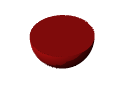
\includegraphics[width=1.6cm]{tableau_geometrie_orbitale_modelisation/S1M0.png} 

& & & & & & \\

& & & \makecell[c]{$1s$} & & & & & &  \\ %centrer la cellule individuellement horizontalement 

\midrule %filet de milieu de tableau

\multirow[t]{4}{*}{$n=2$} & \multirow[t]{2}{*}{$\ell=0$} & \multirow[t]{2}{*}{$2s$} & 
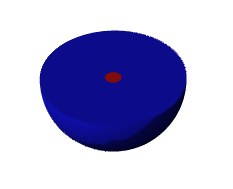
\includegraphics[width=1.6cm]{tableau_geometrie_orbitale_modelisation/S2M0.png} 
& & & & & & \\

& & & \makecell[c]{$2s$} & & & & & &  \\ %centrer la cellule individuellement 

\addlinespace

& \multirow[t]{2}{*}{$\ell=1$} & \multirow[t]{2}{*}{$2p$} & 
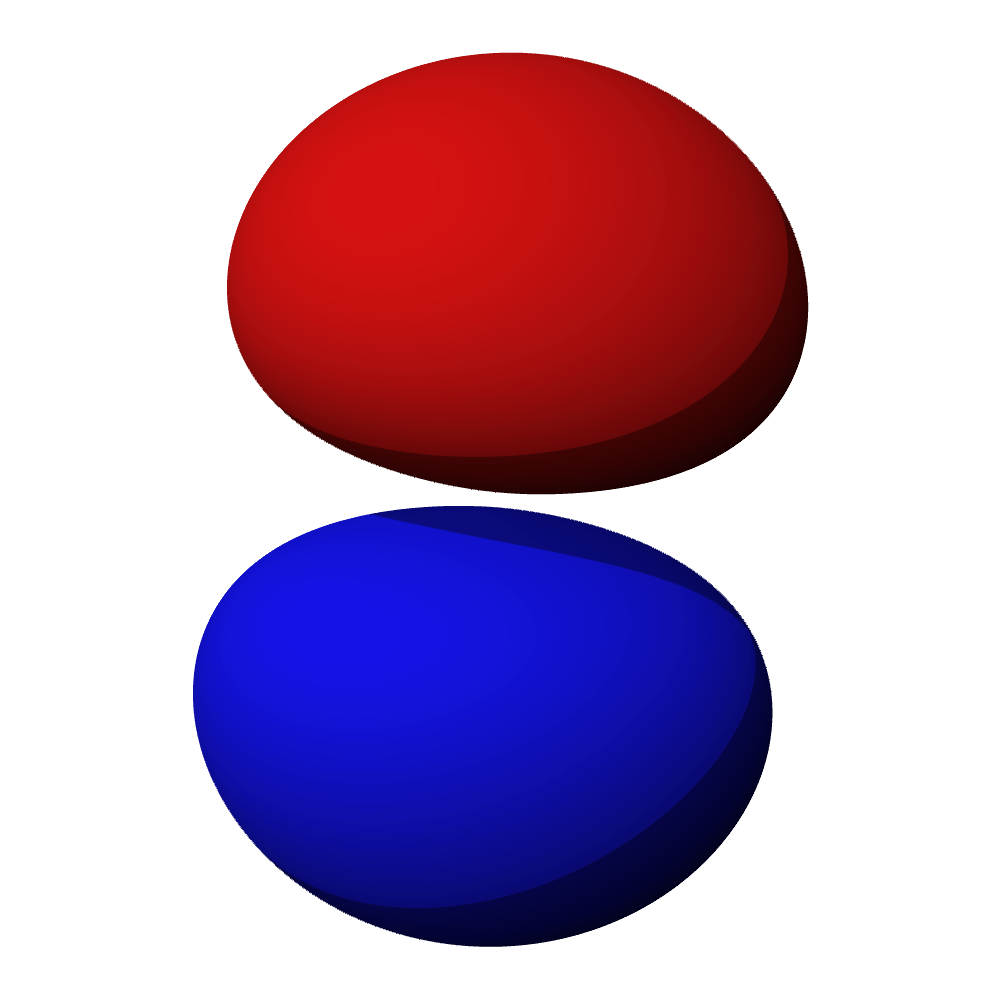
\includegraphics[width=1.6cm]{tableau_geometrie_orbitale_modelisation/Pz_orbital.png} 
&
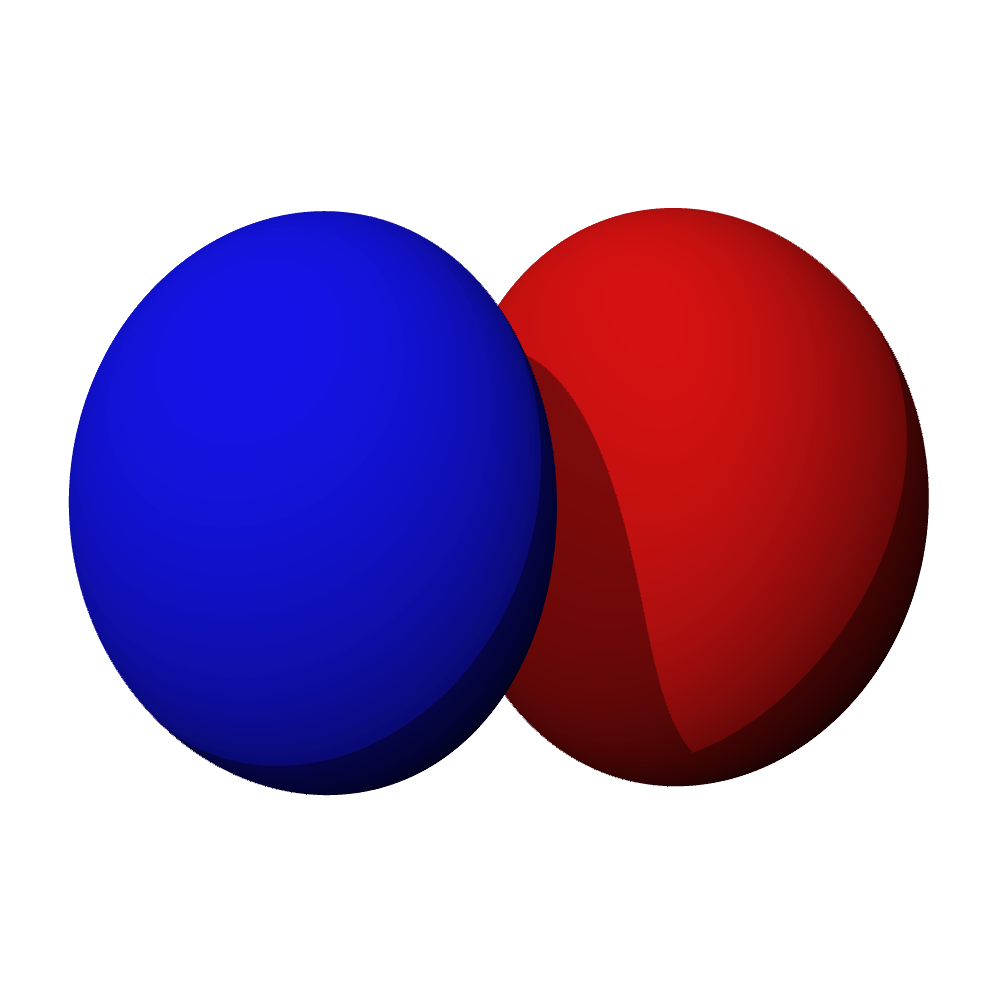
\includegraphics[width=1.6cm]{tableau_geometrie_orbitale_modelisation/Px_orbital.png}  
&
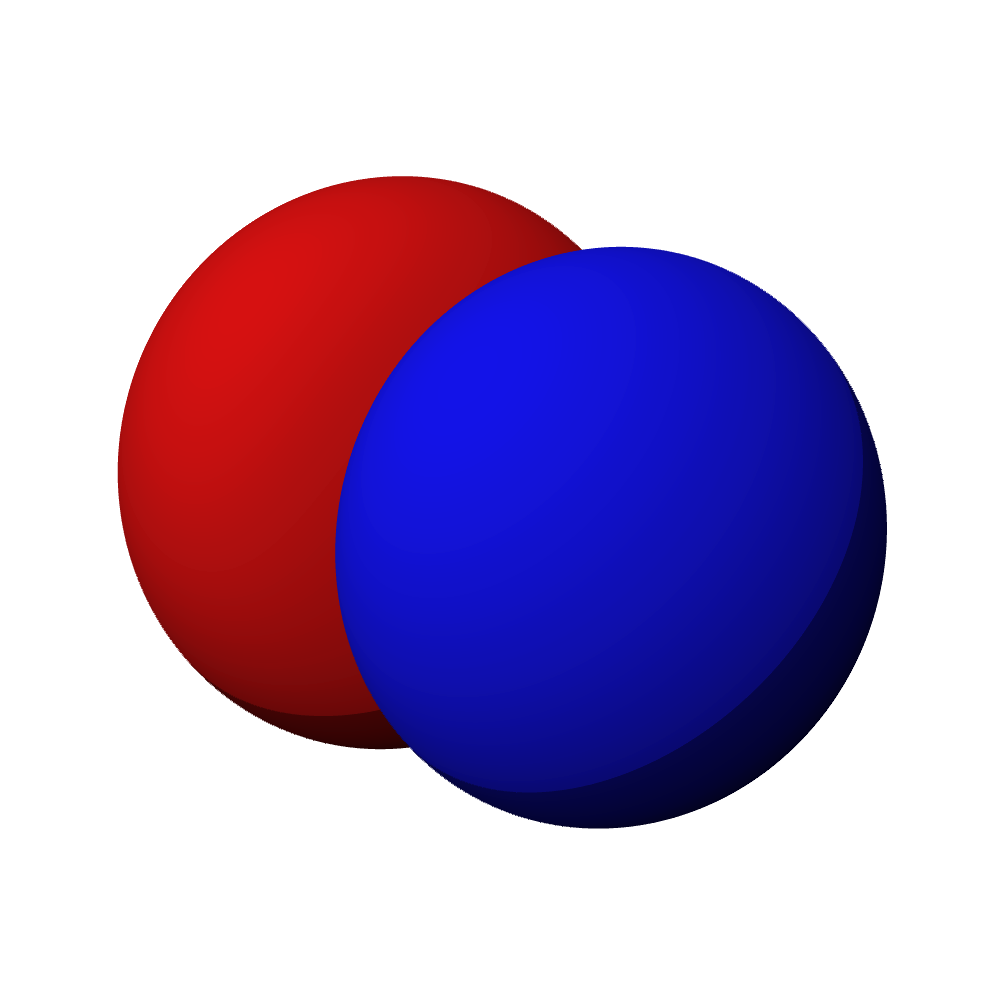
\includegraphics[width=1.6cm]{tableau_geometrie_orbitale_modelisation/Py_orbital.png} 
& & & & \\

& & & \makecell[c]{$2p_z$} & \makecell[c]{$2p_x$} & \makecell[c]{$2p_y$} & & & &  \\ %centrer la cellule individuellement 

\midrule %filet de milieu de tableau

\multirow[t]{6}{*}{$n=3$} & \multirow[t]{2}{*}{$\ell=0$} & \multirow[t]{2}{*}{$3s$} & 
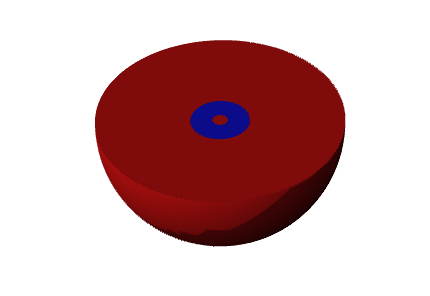
\includegraphics[width=1.6cm]{tableau_geometrie_orbitale_modelisation/S3M0.png} 
& & & & & & \\

& & & \makecell[c]{$3s$} & & & & & &  \\ %centrer la cellule individuellement 

\addlinespace

& \multirow[t]{2}{*}{$\ell=1$} & \multirow[t]{2}{*}{$3p$} & 
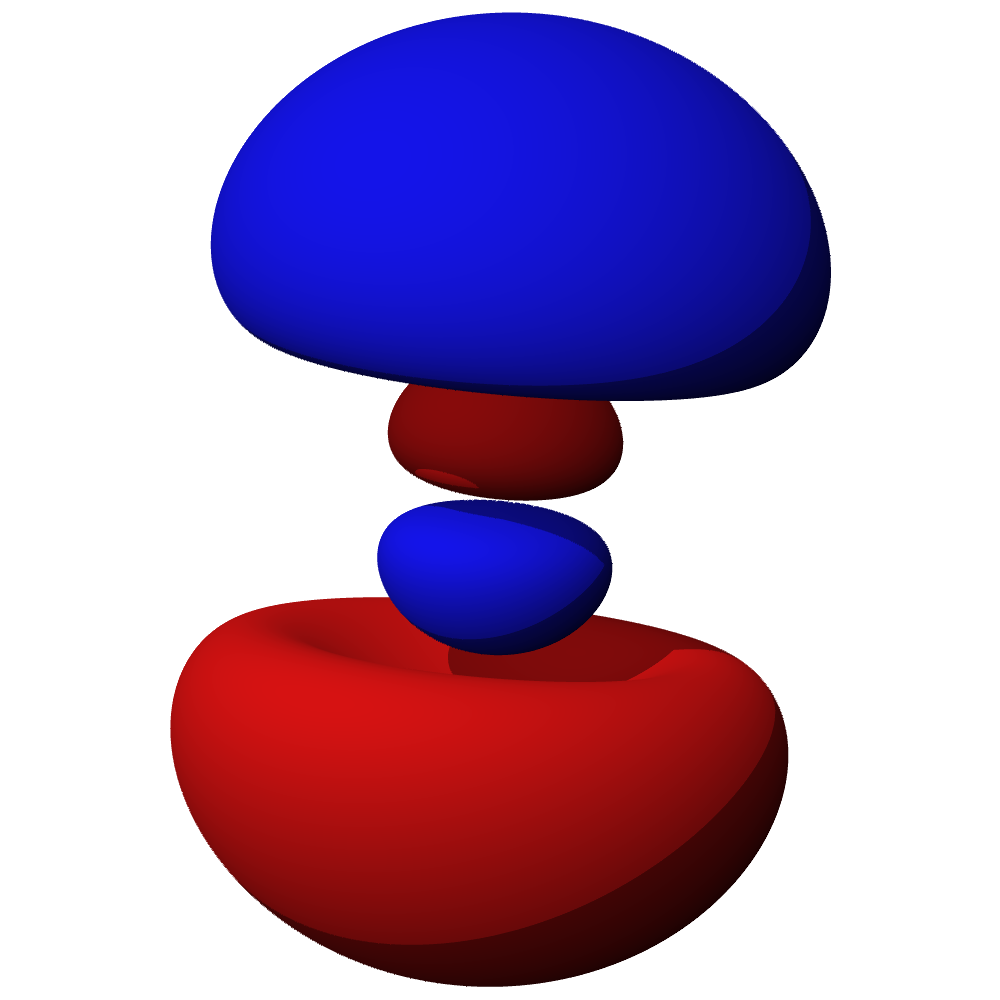
\includegraphics[width=1.6cm]{tableau_geometrie_orbitale_modelisation/P3z.png} 
&
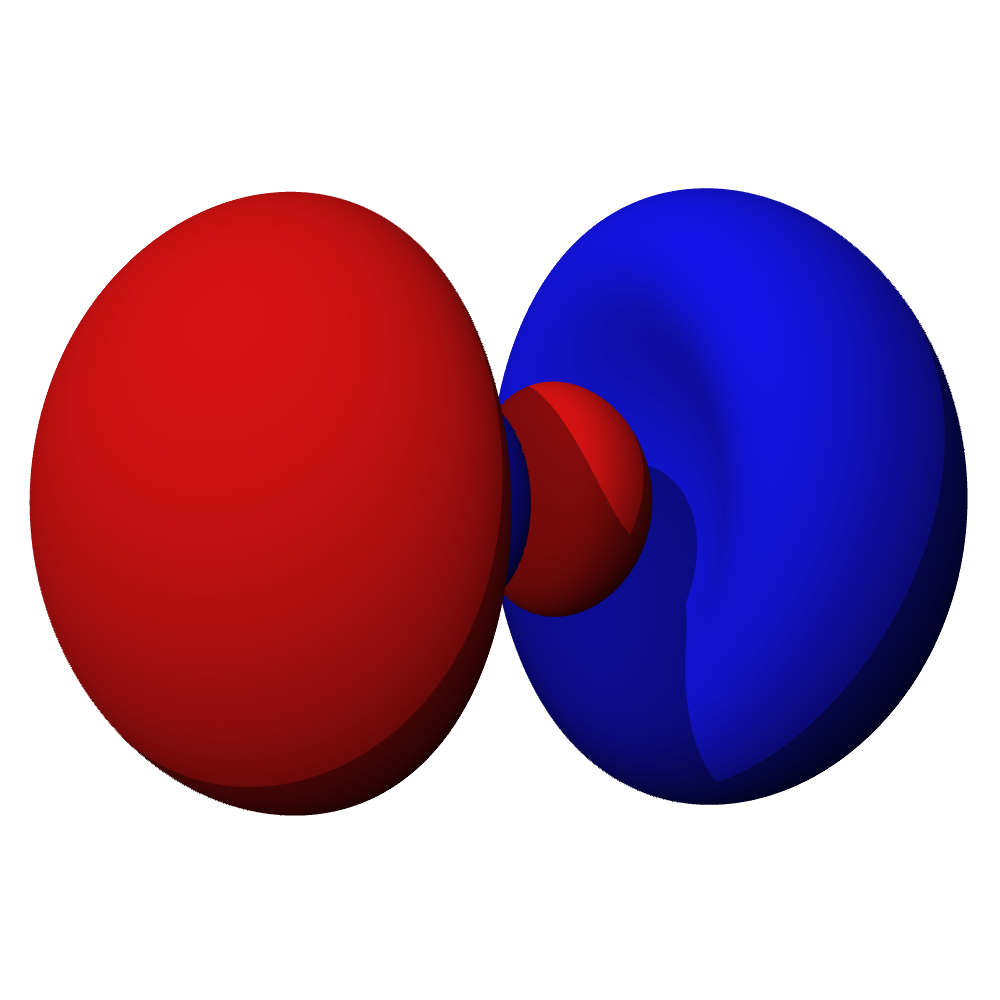
\includegraphics[width=1.6cm]{tableau_geometrie_orbitale_modelisation/P3x.png}  
&
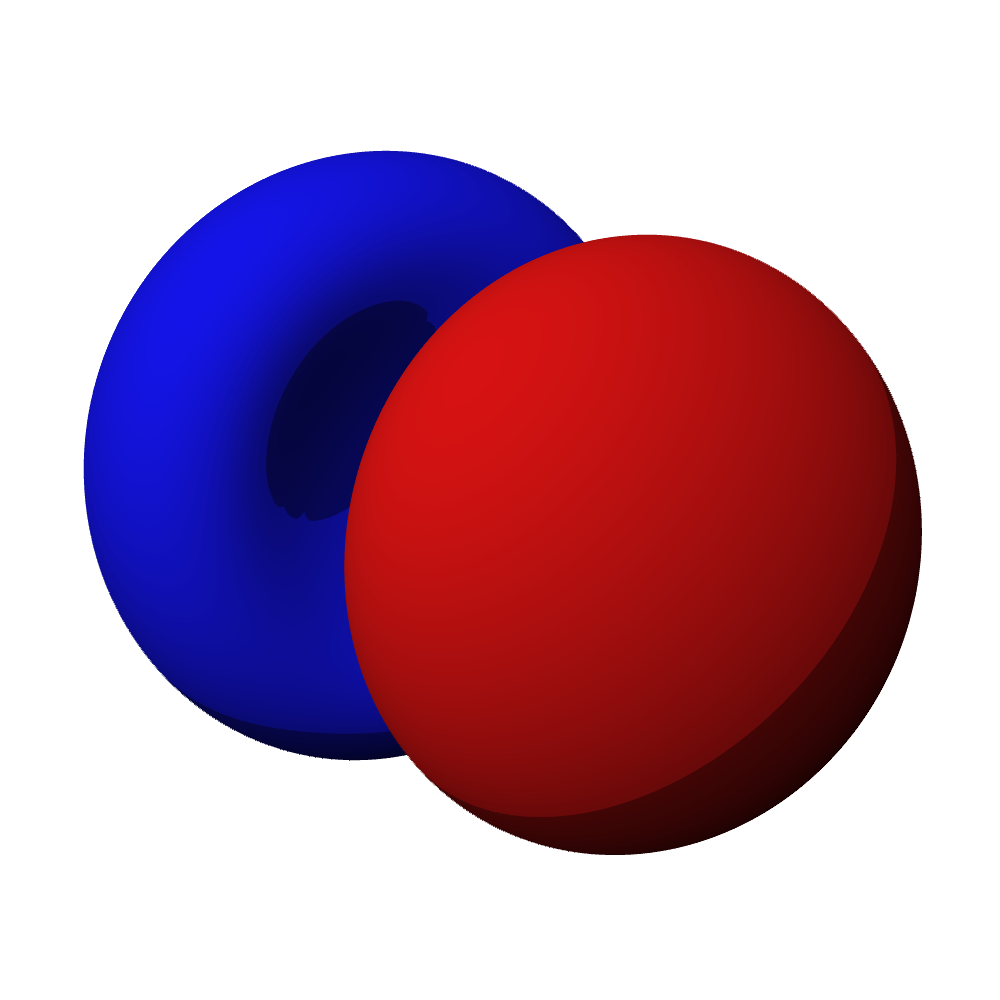
\includegraphics[width=1.6cm]{tableau_geometrie_orbitale_modelisation/P3y.png} 
& & & & \\

& & & \makecell[c]{$3p_z$} & \makecell[c]{$3p_x$} & \makecell[c]{$3p_y$} & & & &  \\ %centrer la cellule individuellement 

\addlinespace

 & \multirow[t]{2}{*}{$\ell=2$} & \multirow[t]{2}{*}{$3d$} & 
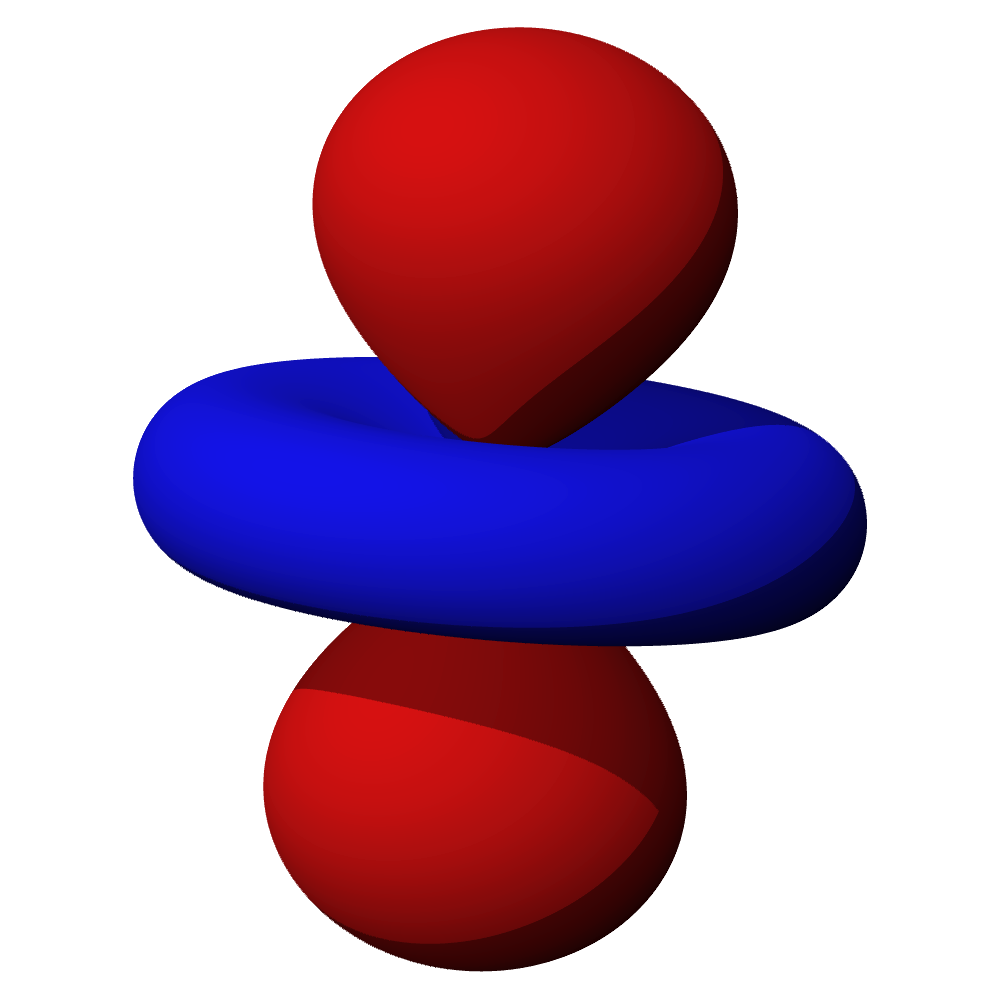
\includegraphics[width=1.6cm]{tableau_geometrie_orbitale_modelisation/Dz2_orbital.png} 
&
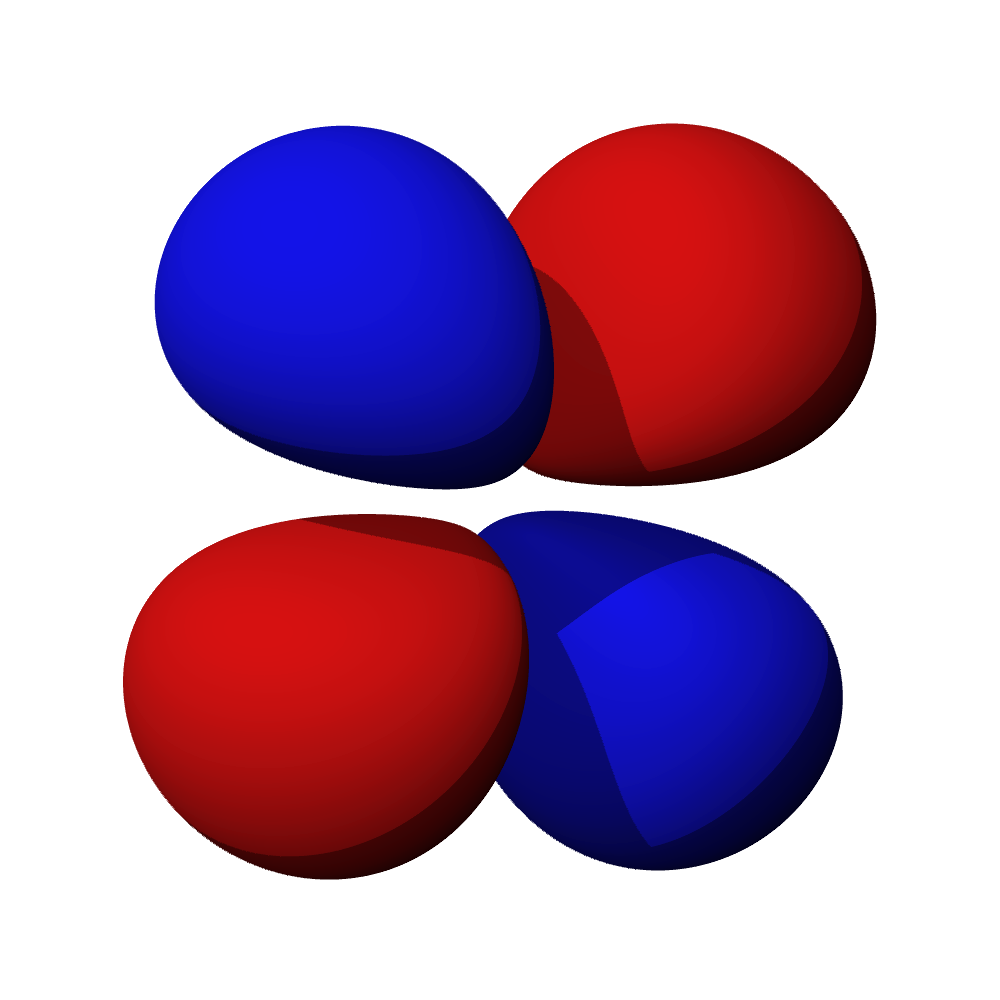
\includegraphics[width=1.6cm]{tableau_geometrie_orbitale_modelisation/Dxz_orbital.png}  
&
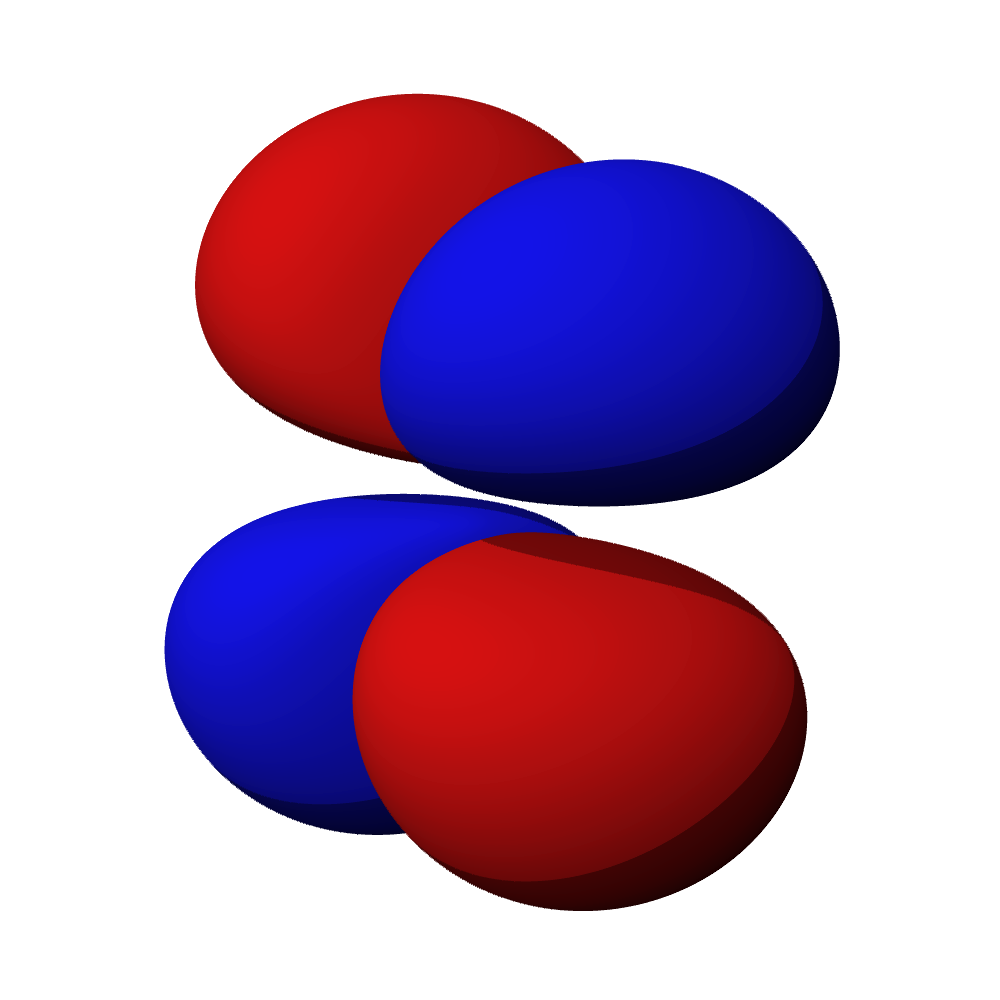
\includegraphics[width=1.6cm]{tableau_geometrie_orbitale_modelisation/Dyz_orbital.png} 
& 
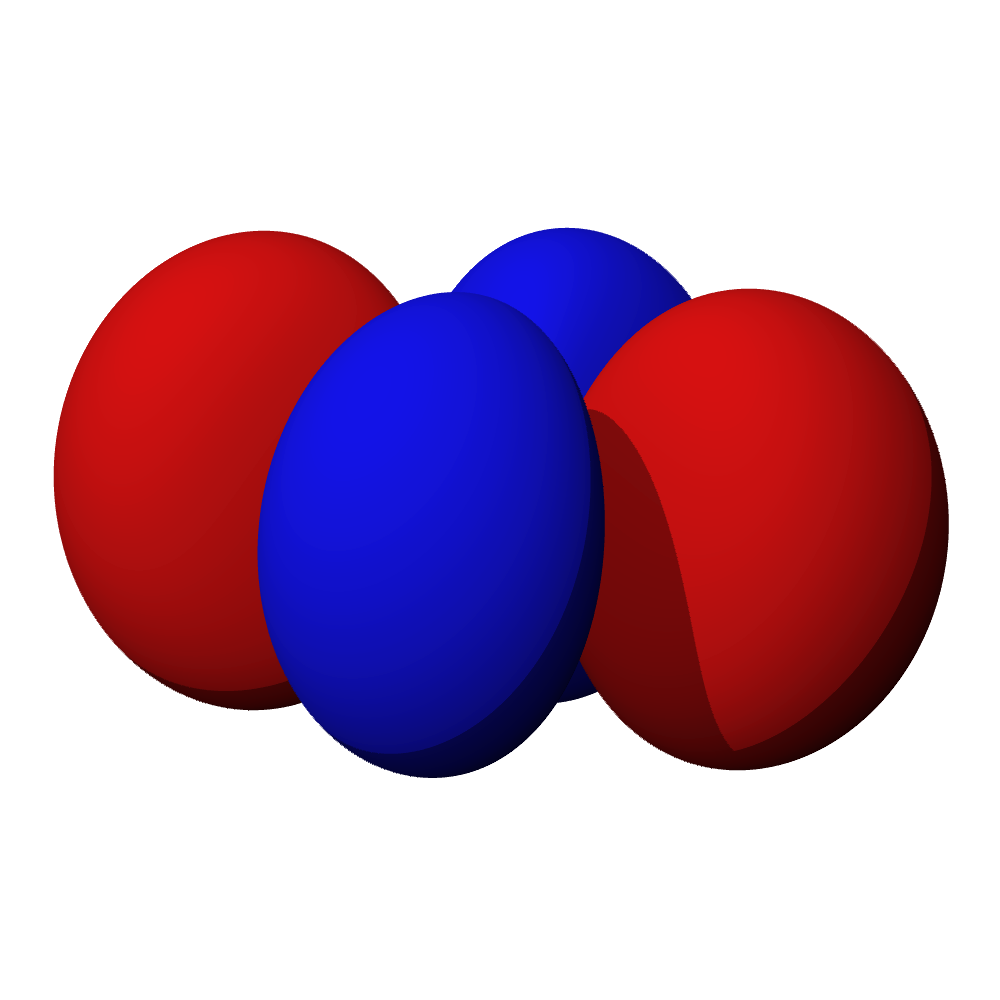
\includegraphics[width=1.6cm]{tableau_geometrie_orbitale_modelisation/Dxy_orbital.png} 
&
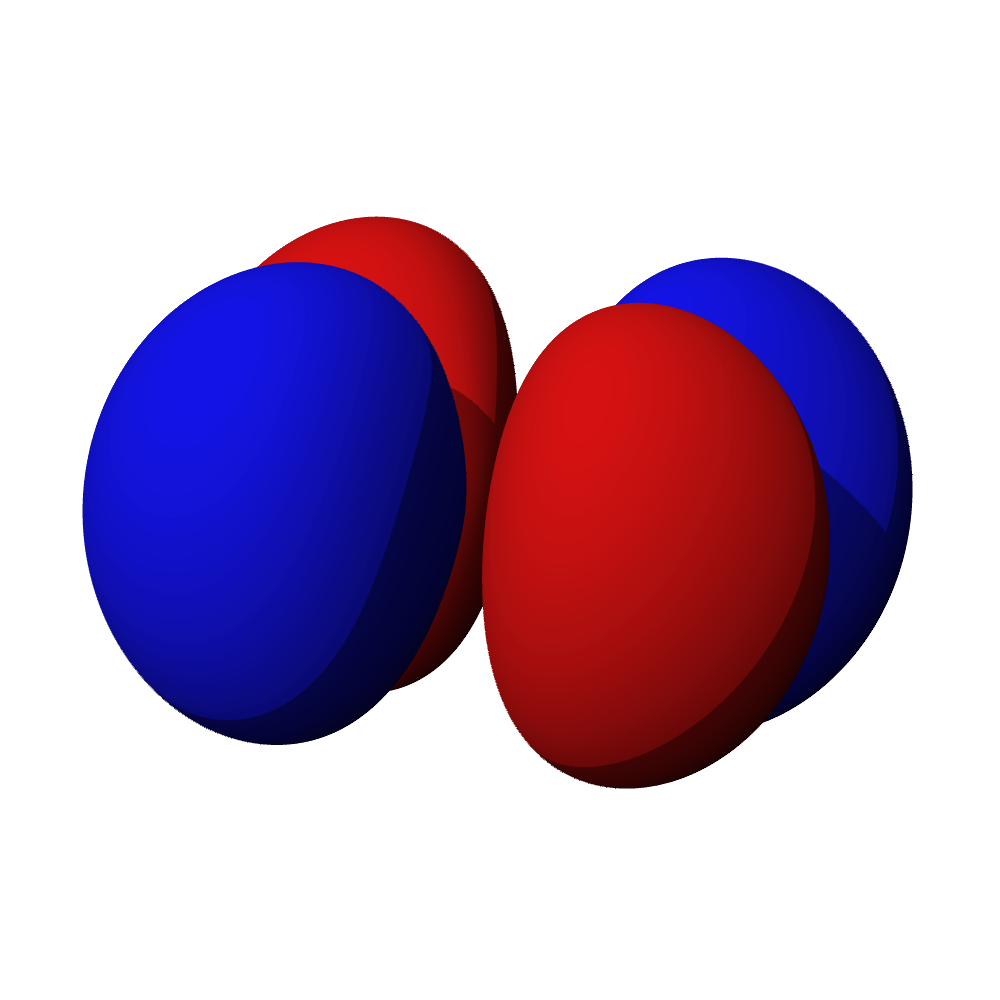
\includegraphics[width=1.6cm]{tableau_geometrie_orbitale_modelisation/Dx2-y2_orbital.png} 
& & \\
& & & \makecell[c]{$3d_{z^2}$} & \makecell[c]{$3d_{xz}$} & \makecell[c]{$3d_{yz}$} & \makecell[c]{$3d_{xy}$} & \makecell[c]{$3d_{x^{2}-y^{2}}$} & &  \\ %centrer la cellule individuellement 

\addlinespace

%\noalign{\break} %impose le saut de page au tableau tout en répartissant verticalement le tableau

\multirow[t]{8}{*}{$n=4$} & \multirow[t]{2}{*}{$\ell=0$} & \multirow[t]{2}{*}{$4s$} & 
\centering
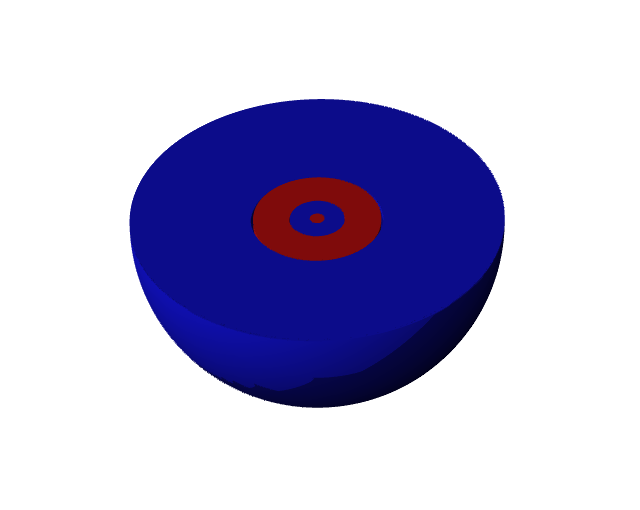
\includegraphics[width=1.6cm]{tableau_geometrie_orbitale_modelisation/S4M0.png} 
& & & & & & \\

& & & \makecell[c]{$3s$} & & & & & &  \\ %centrer la cellule individuellement 

\addlinespace

& \multirow[t]{2}{*}{$\ell=1$} & \multirow[t]{2}{*}{$4p$} & 
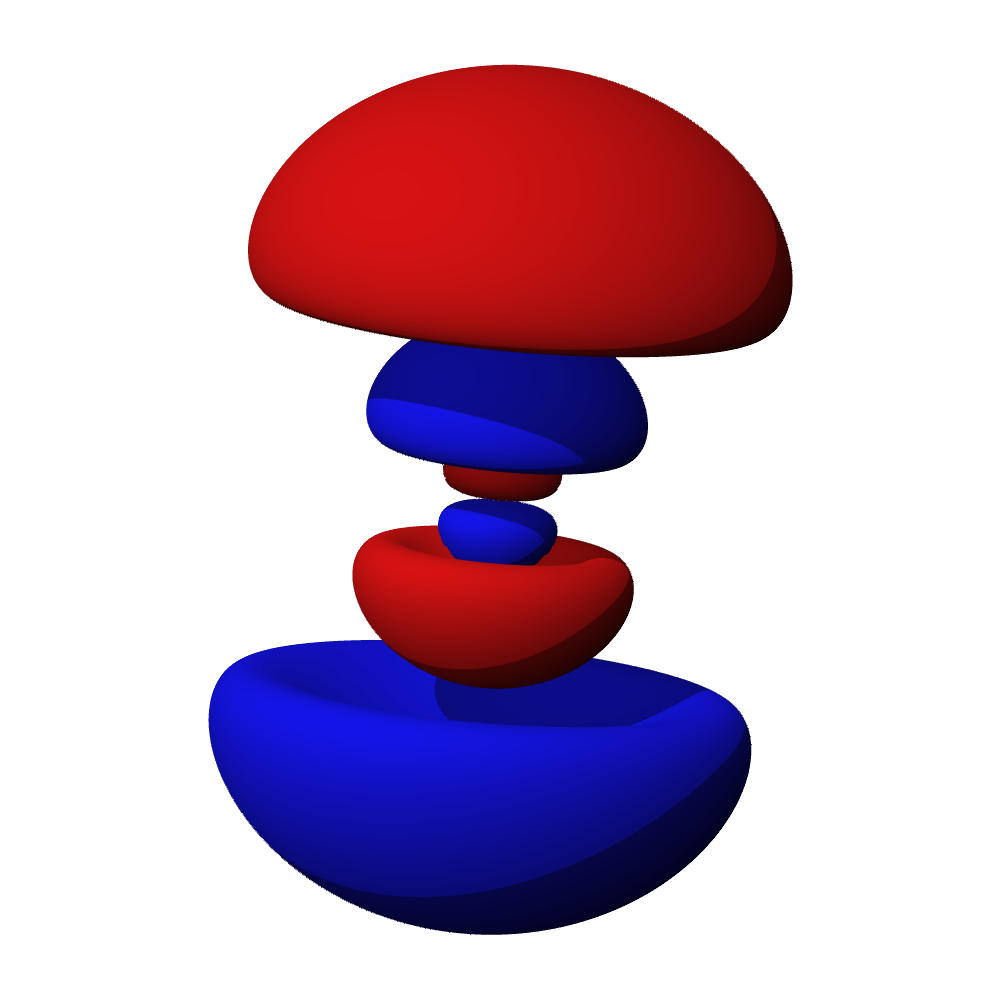
\includegraphics[width=1.6cm]{tableau_geometrie_orbitale_modelisation/P4z.png} 
&
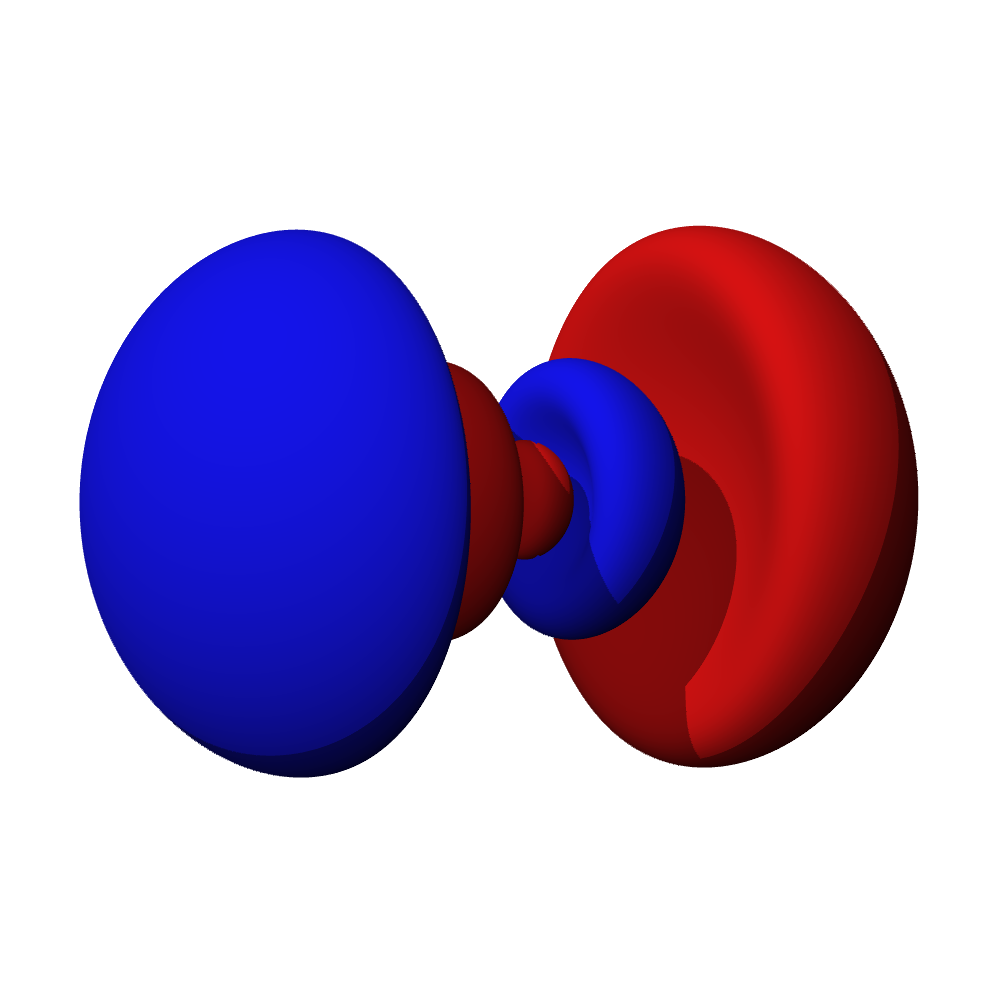
\includegraphics[width=1.6cm]{tableau_geometrie_orbitale_modelisation/P4x.png}  
&
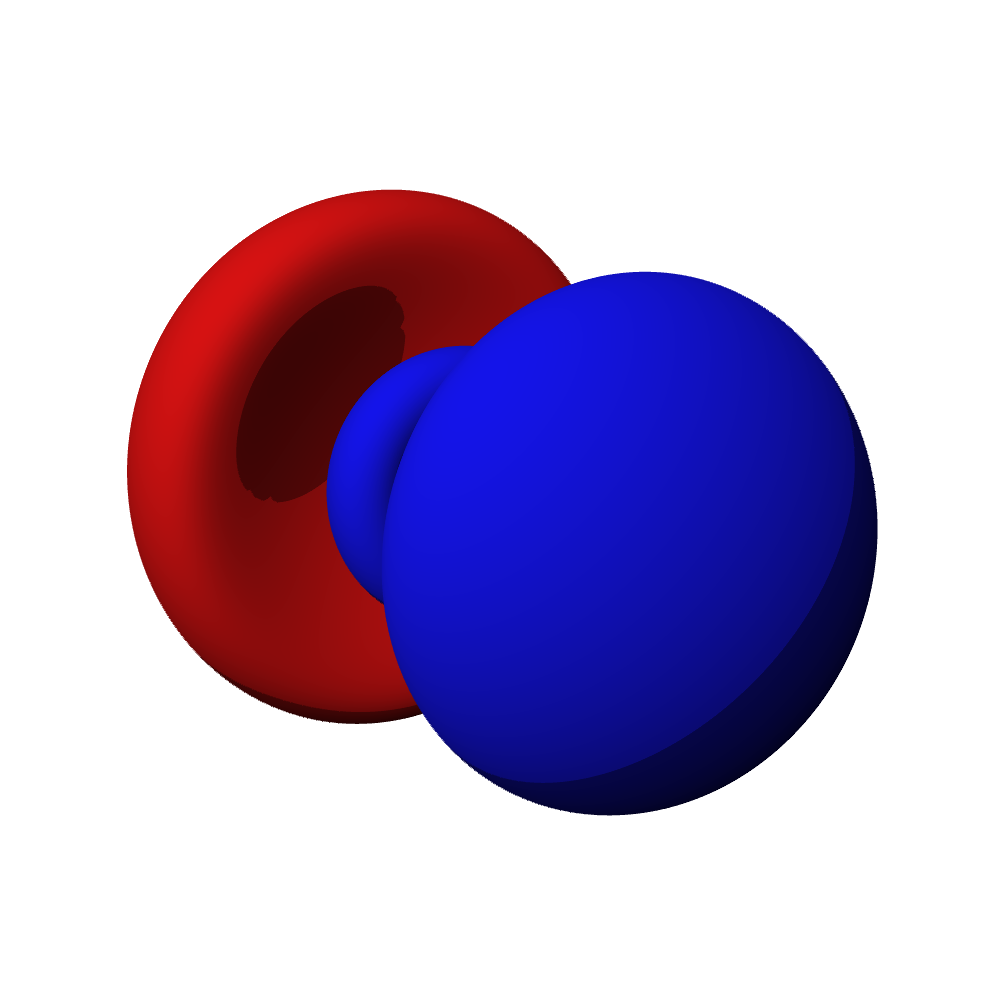
\includegraphics[width=1.6cm]{tableau_geometrie_orbitale_modelisation/P4y.png} 
& & & & \\

& & & \makecell[c]{$3p_z$} & \makecell[c]{$3p_x$} & \makecell[c]{$3p_y$} & & & &  \\ %centrer la cellule individuellement 

\addlinespace

& \multirow[t]{2}{*}{$\ell=2$} & \multirow[t]{2}{*}{$4d$} & 
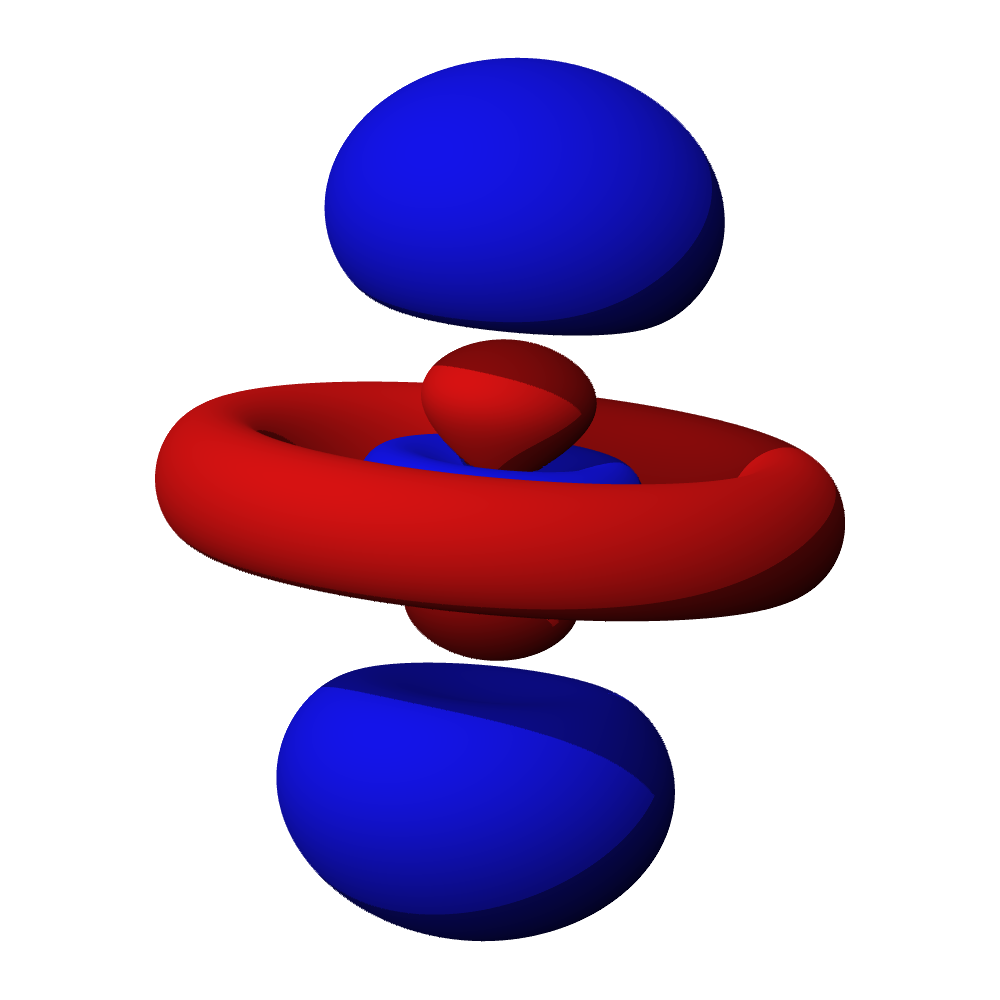
\includegraphics[width=1.6cm]{tableau_geometrie_orbitale_modelisation/D4z2.png} 
&
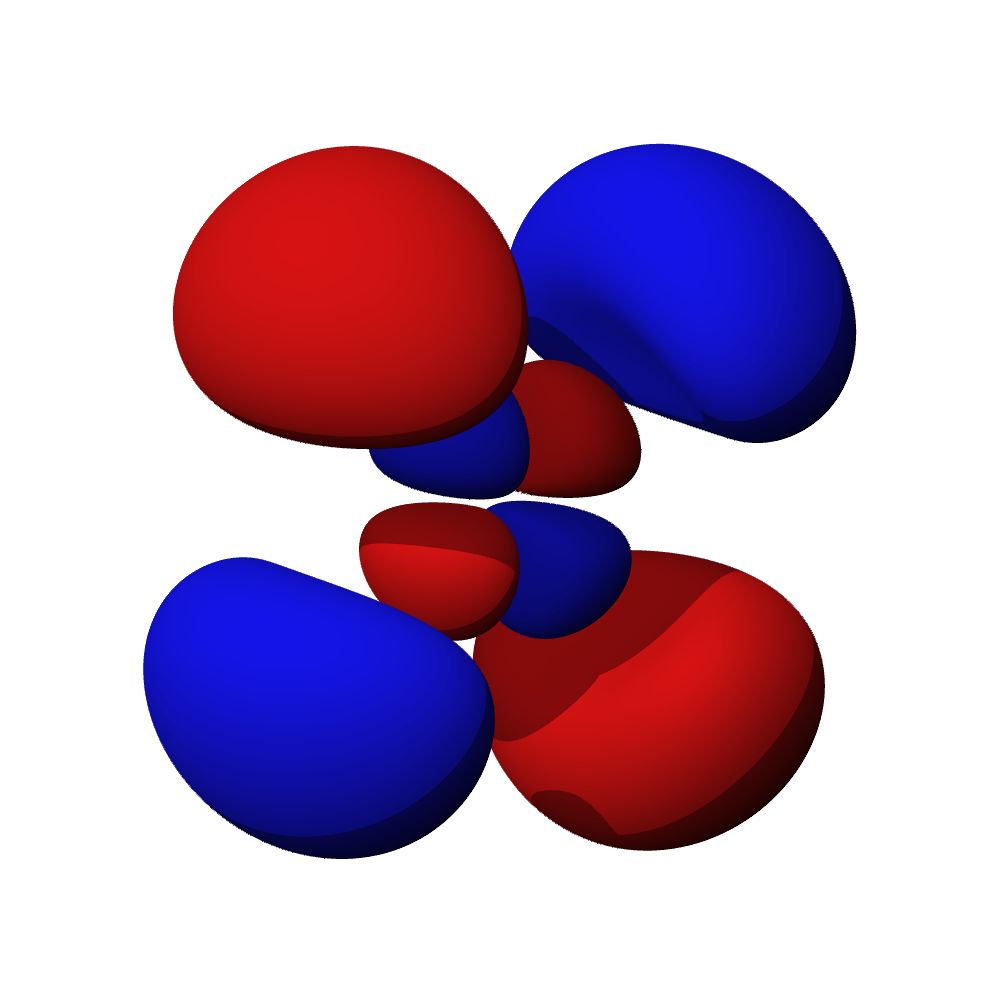
\includegraphics[width=1.6cm]{tableau_geometrie_orbitale_modelisation/D4xz.png}  
&
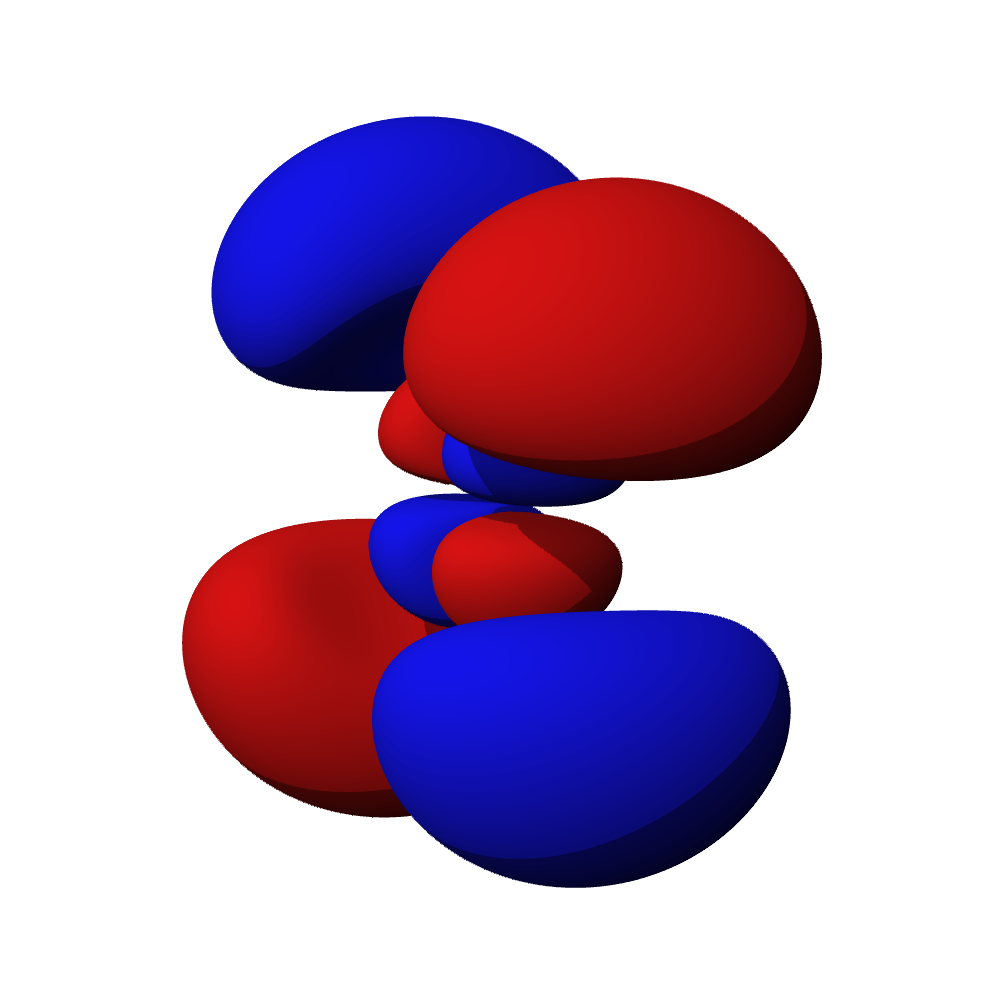
\includegraphics[width=1.6cm]{tableau_geometrie_orbitale_modelisation/D4yz.png} 
& 
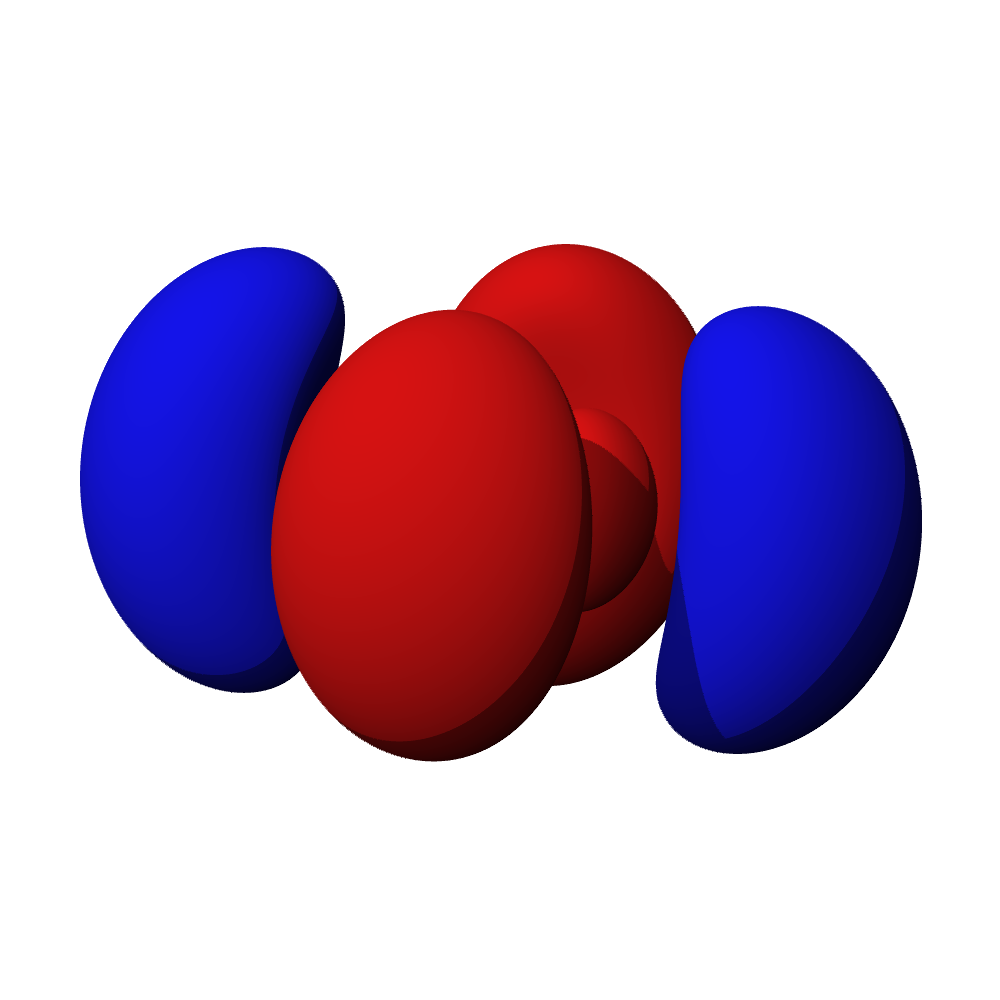
\includegraphics[width=1.6cm]{tableau_geometrie_orbitale_modelisation/D4xy.png} 
&
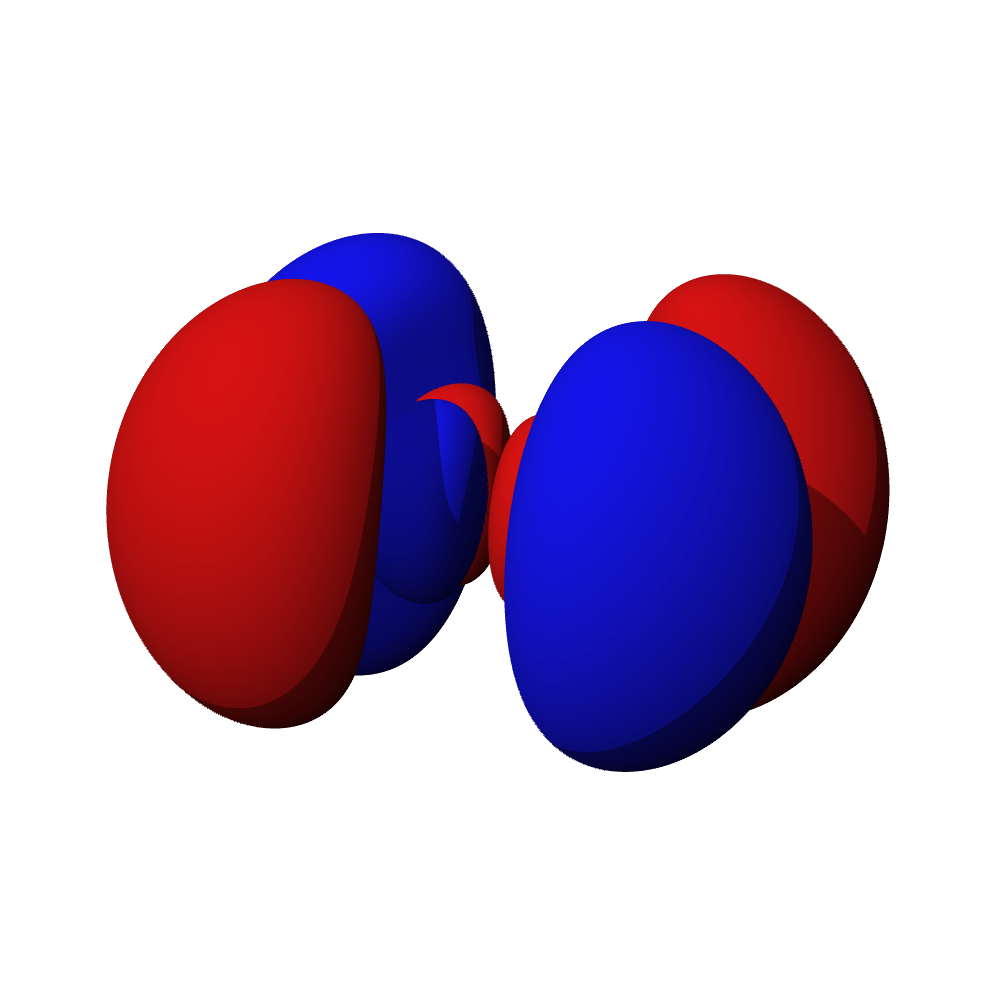
\includegraphics[width=1.6cm]{tableau_geometrie_orbitale_modelisation/D4x2-y2.png} 
& & \\

& & & \makecell[c]{$3d_{z^2}$} & \makecell[c]{$3d_{xz}$} & \makecell[c]{$3d_{yz}$} & \makecell[c]{$3d_{xy}$} & \makecell[c]{$3d_{x^{2}-y^{2}}$} & &  \\ %centrer la cellule individuellement 

\addlinespace

& \multirow[t]{2}{*}{$\ell=3$} & \multirow[t]{2}{*}{$4f$} & 
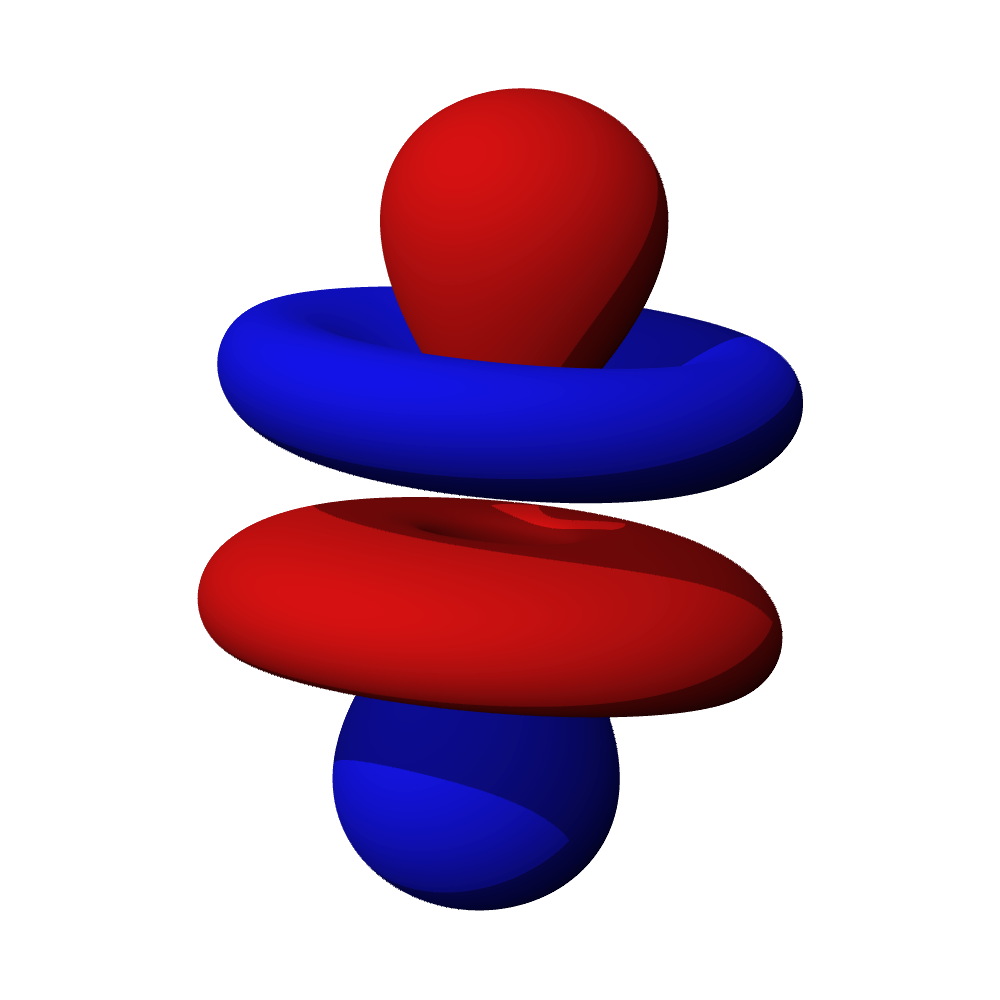
\includegraphics[width=1.6cm]{tableau_geometrie_orbitale_modelisation/Fz3_orbital.png} 
&
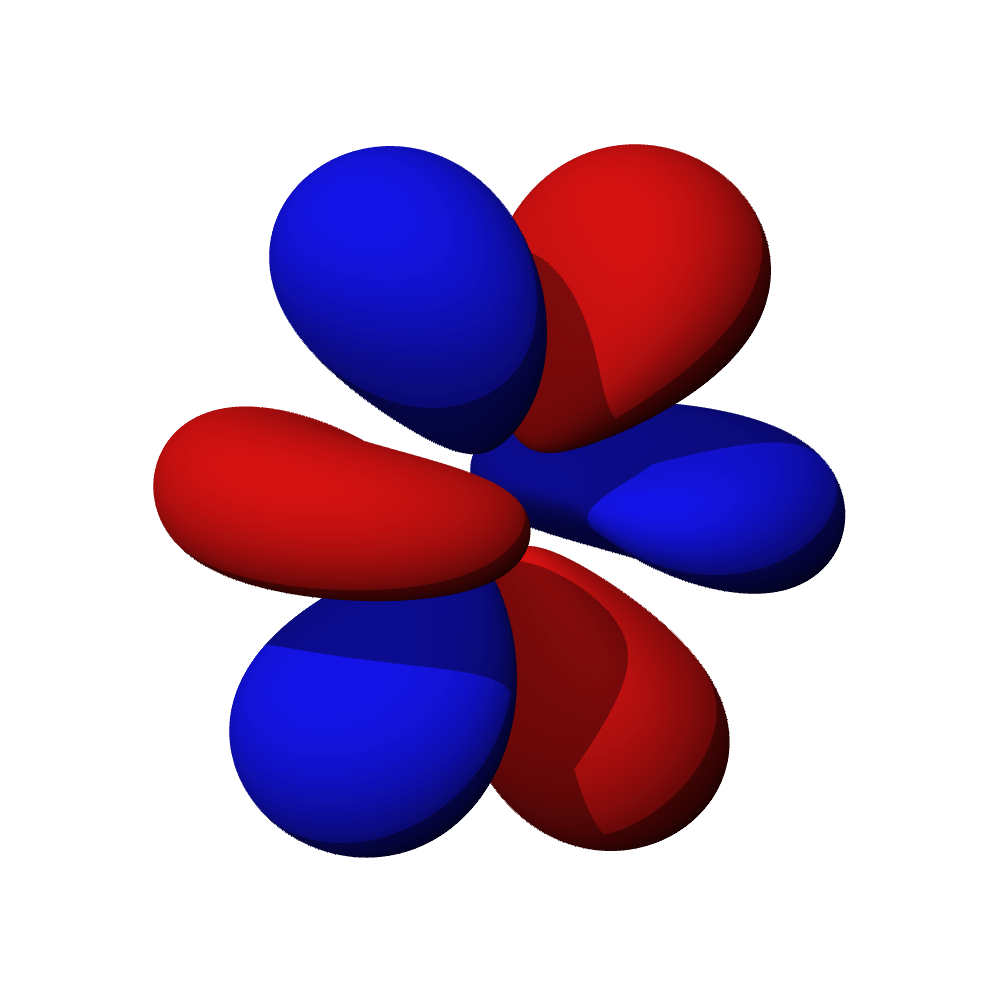
\includegraphics[width=1.6cm]{tableau_geometrie_orbitale_modelisation/Fxz2_orbital.png}  
&
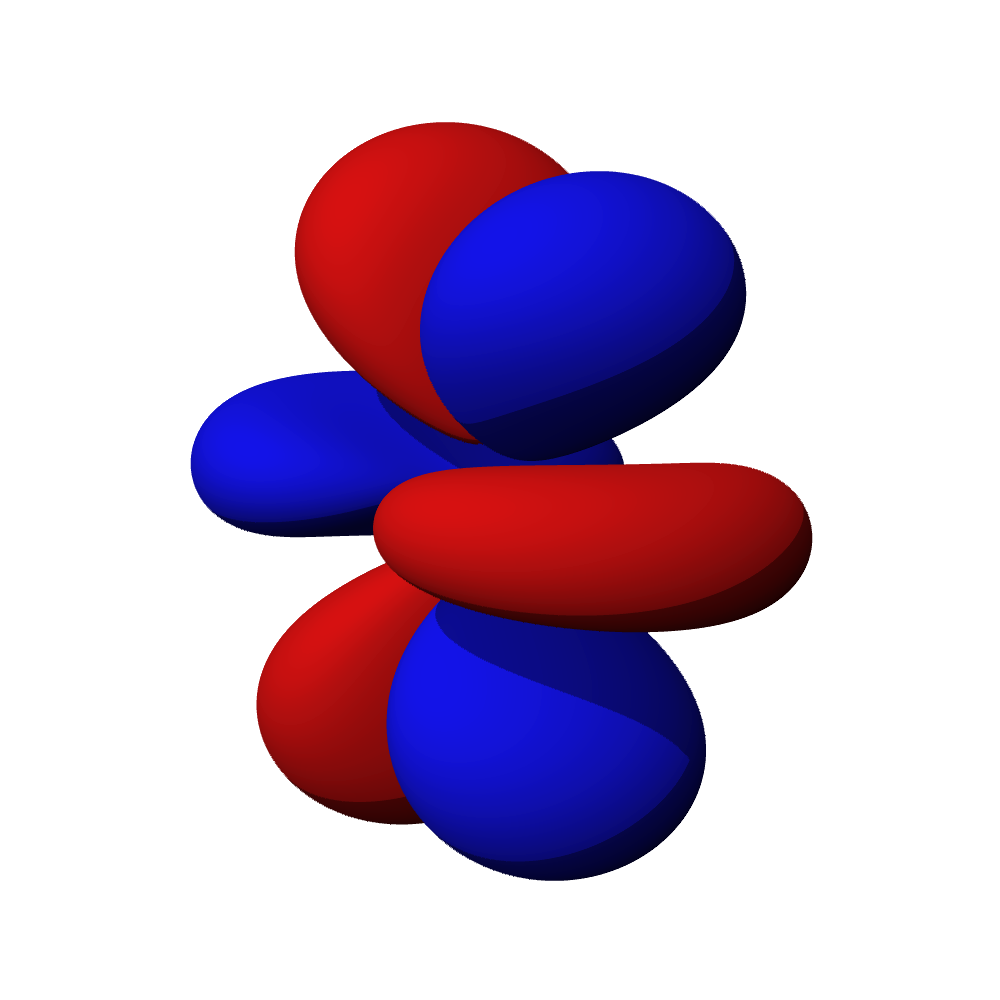
\includegraphics[width=1.6cm]{tableau_geometrie_orbitale_modelisation/Fyz2_orbital.png} 
& 
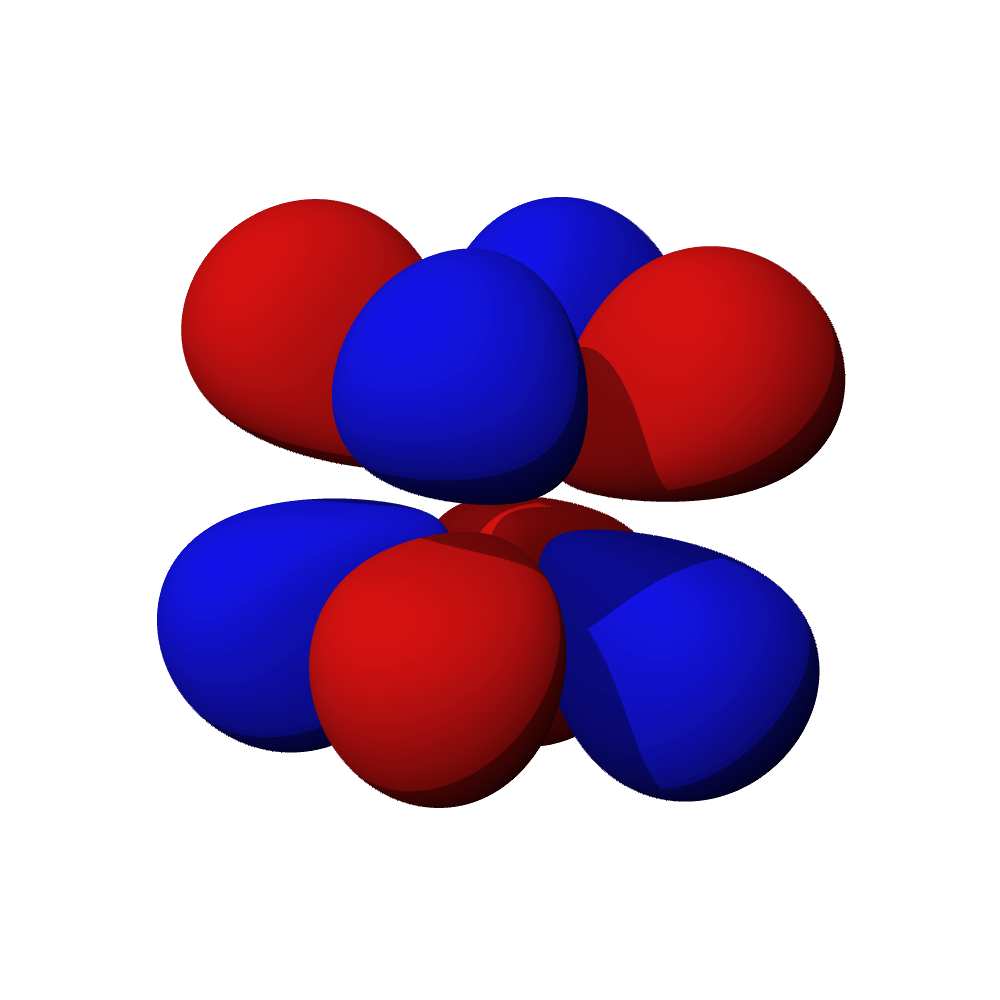
\includegraphics[width=1.6cm]{tableau_geometrie_orbitale_modelisation/Fxyz_orbital.png} 
&
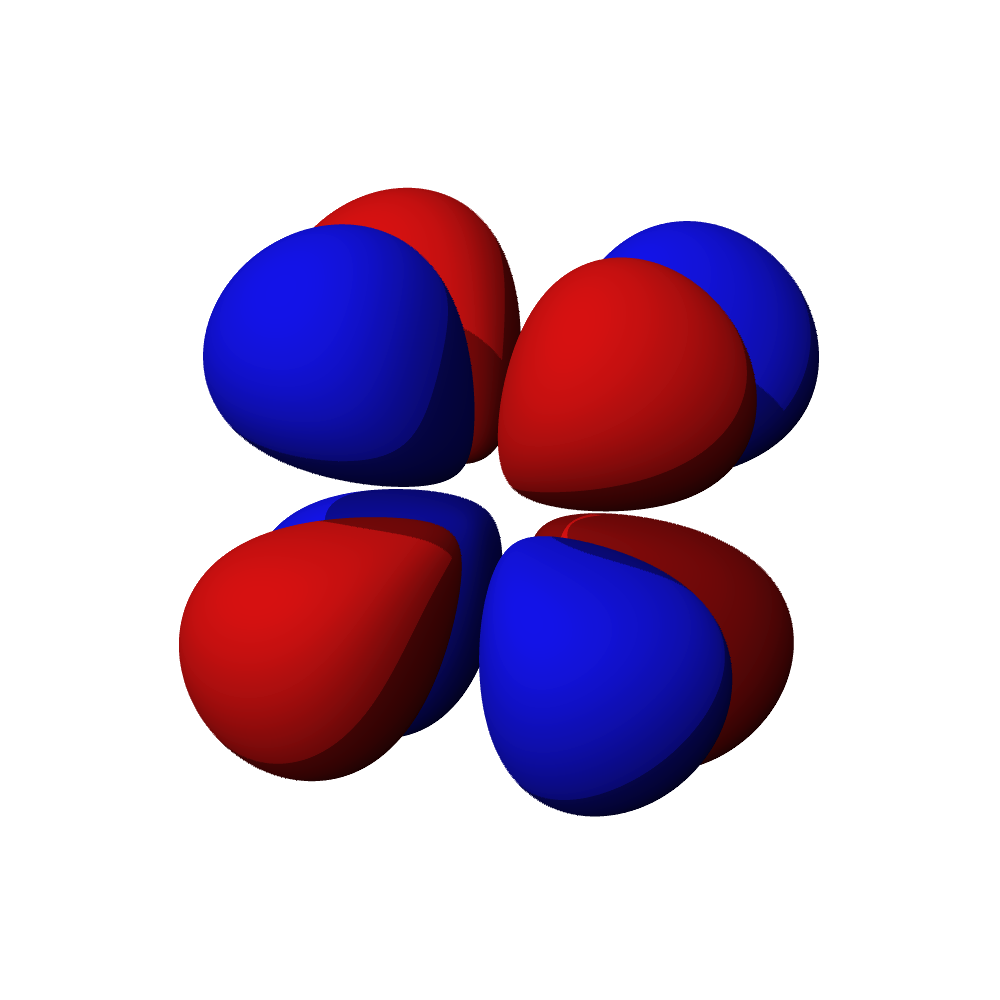
\includegraphics[width=1.6cm]{tableau_geometrie_orbitale_modelisation/Fz(x2-y2)_orbital.png} 
& 
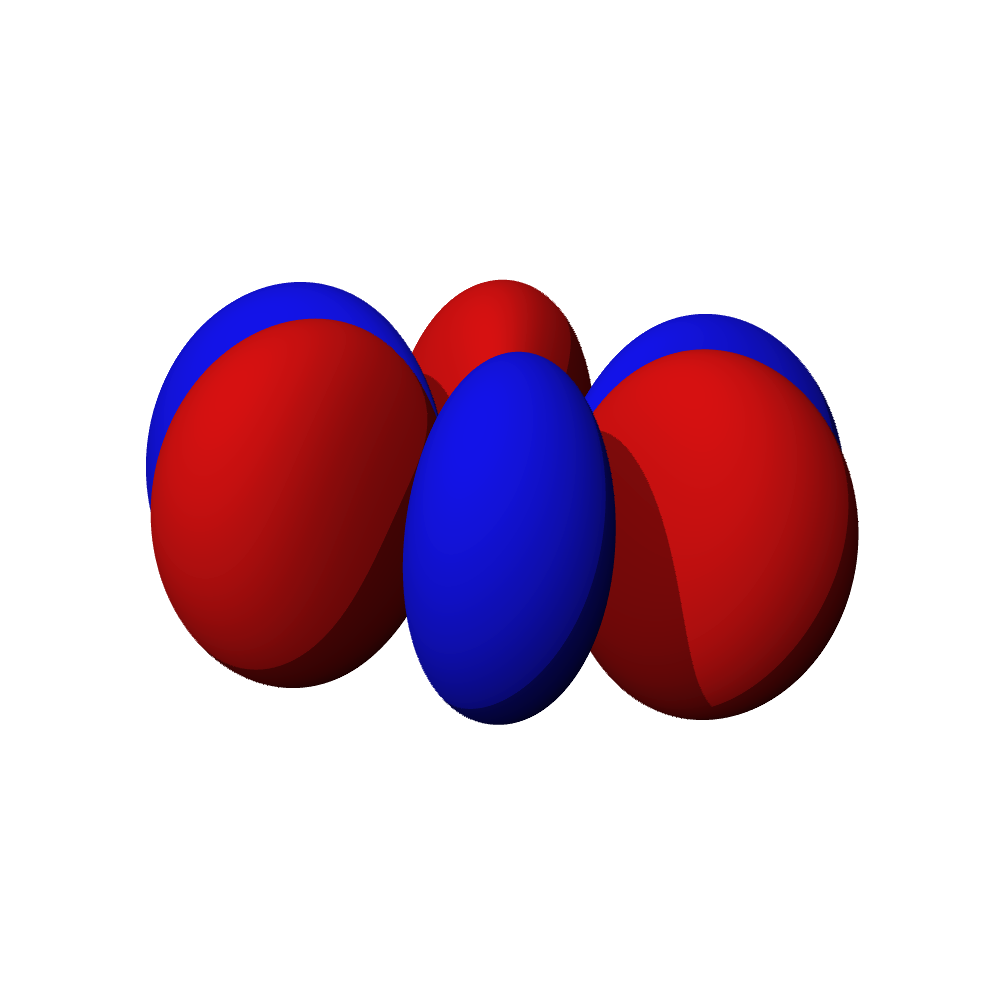
\includegraphics[width=1.6cm]{tableau_geometrie_orbitale_modelisation/Fx(x2-3y2)_orbital.png}
&
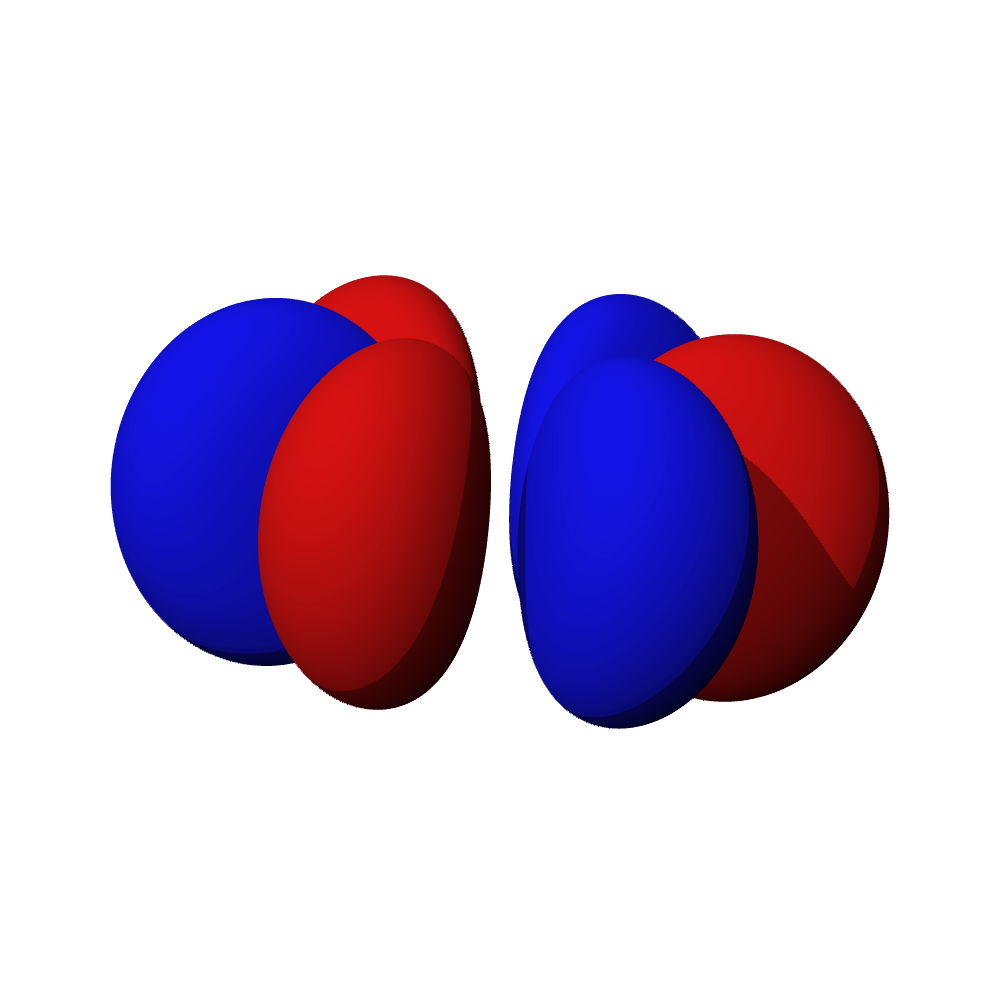
\includegraphics[width=1.6cm]{tableau_geometrie_orbitale_modelisation/Fy(3x2-y2)_orbital.png} \\

& & & \makecell[c]{$4f_{z^3}$} & \makecell[c]{$4f_{xz^2}$} & \makecell[c]{$4f_{yz^2}$} & \makecell[c]%
{$4f_{xyz}$} & \makecell[c]{$4f_{z(x^{2}-y^2)}$} & \makecell[c]{$4f_{x(x^{2}-y^2)}$} & \makecell[c]%
{$4f_{y(x^{2}-y^2)}$} \\ %centrer la cellule individuellement 

\midrule %filet de milieu de tableau

\multirow[t]{4}{*}{$n=5$} & \multirow[t]{2}{*}{$\ell=0$} & \multirow[t]{2}{*}{$5s$} & 
\centering
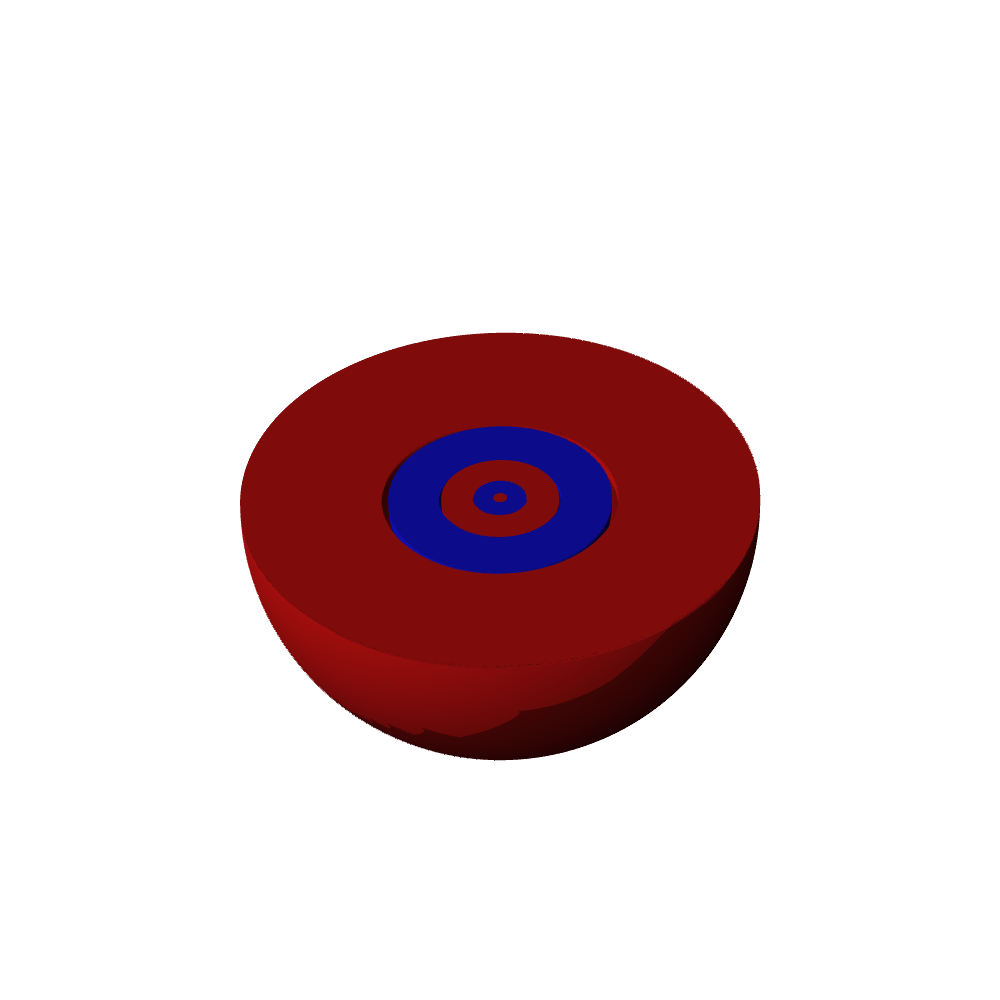
\includegraphics[width=1.6cm]{tableau_geometrie_orbitale_modelisation/S5M0.png} 
& & & & & & \\

& & & \makecell[c]{$5s$} & & & & & &  \\ %centrer la cellule individuellement 

\addlinespace

& \multirow[t]{2}{*}{$\ell=1$} & \multirow[t]{2}{*}{$5p$} & 
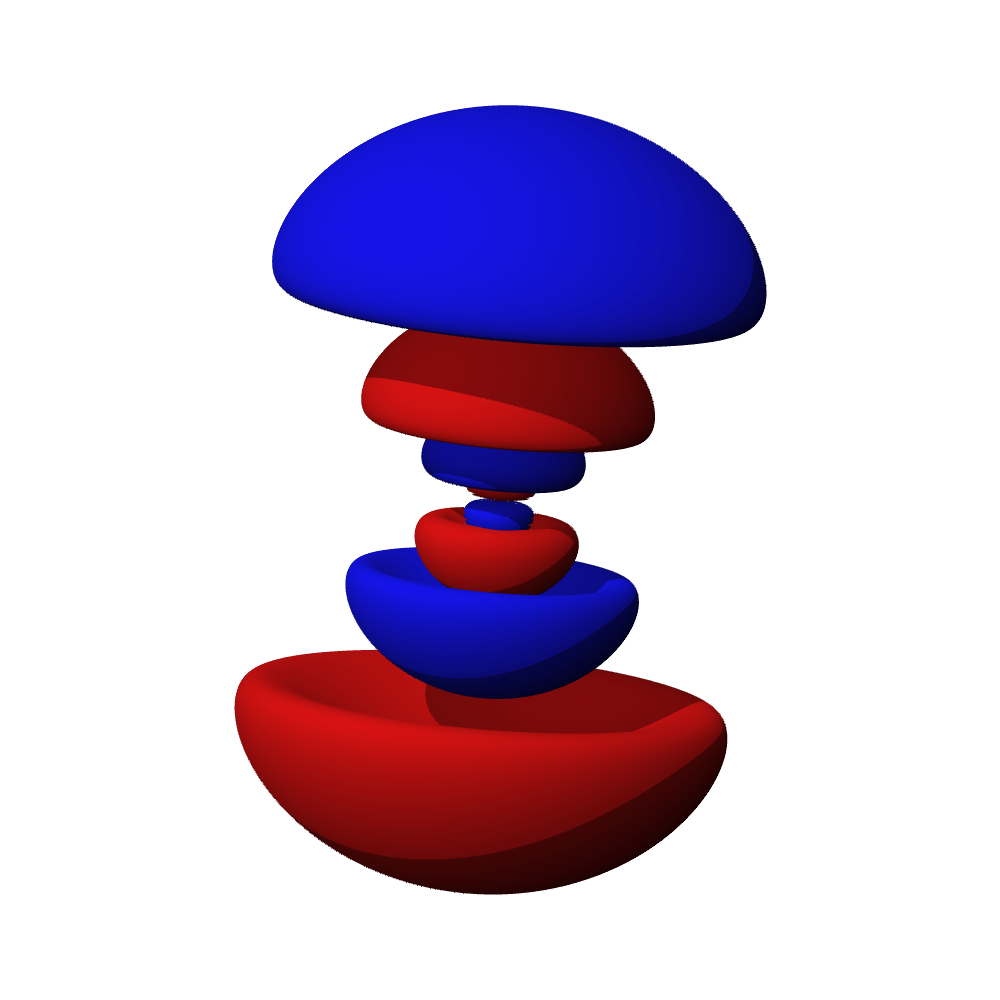
\includegraphics[width=1.6cm]{tableau_geometrie_orbitale_modelisation/P5z.png} 
&
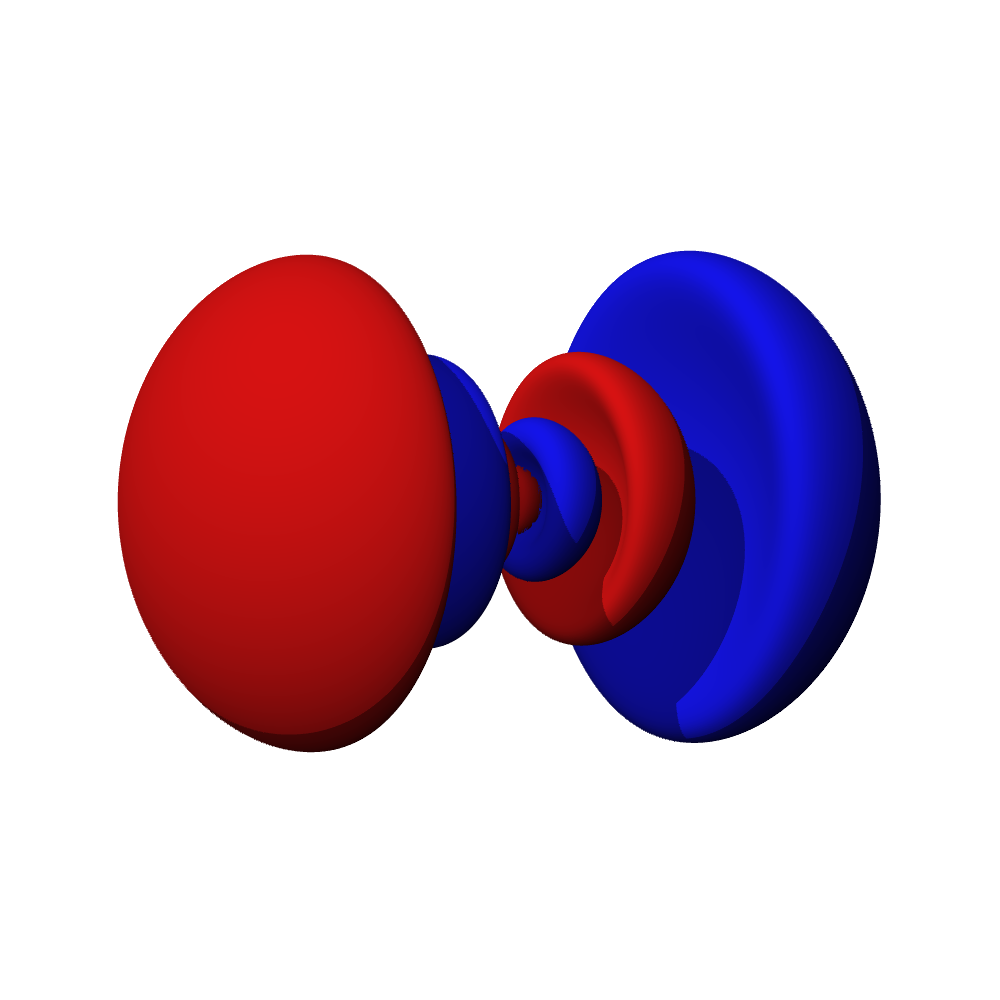
\includegraphics[width=1.6cm]{tableau_geometrie_orbitale_modelisation/P5x.png}  
&
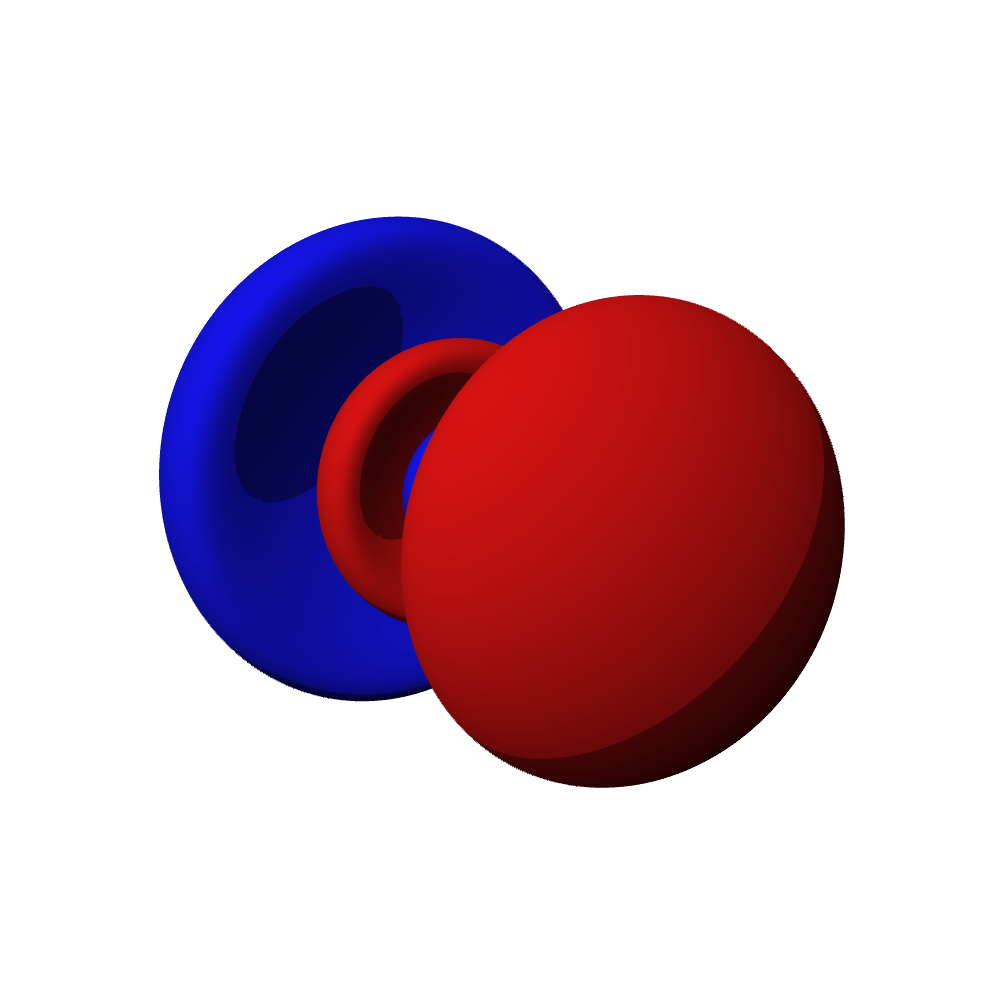
\includegraphics[width=1.6cm]{tableau_geometrie_orbitale_modelisation/P5y.png} 
& & & & \\

& & & \makecell[c]{$5p_z$} & \makecell[c]{$5p_x$} & \makecell[c]{$5p_y$} & & & &  \\ %centrer la cellule individuellement 

\addlinespace

\multirow[t]{2}{*}{$n=5$} & \multirow[t]{2}{*}{$\ell=2$} & \multirow[t]{2}{*}{$5d$} & 
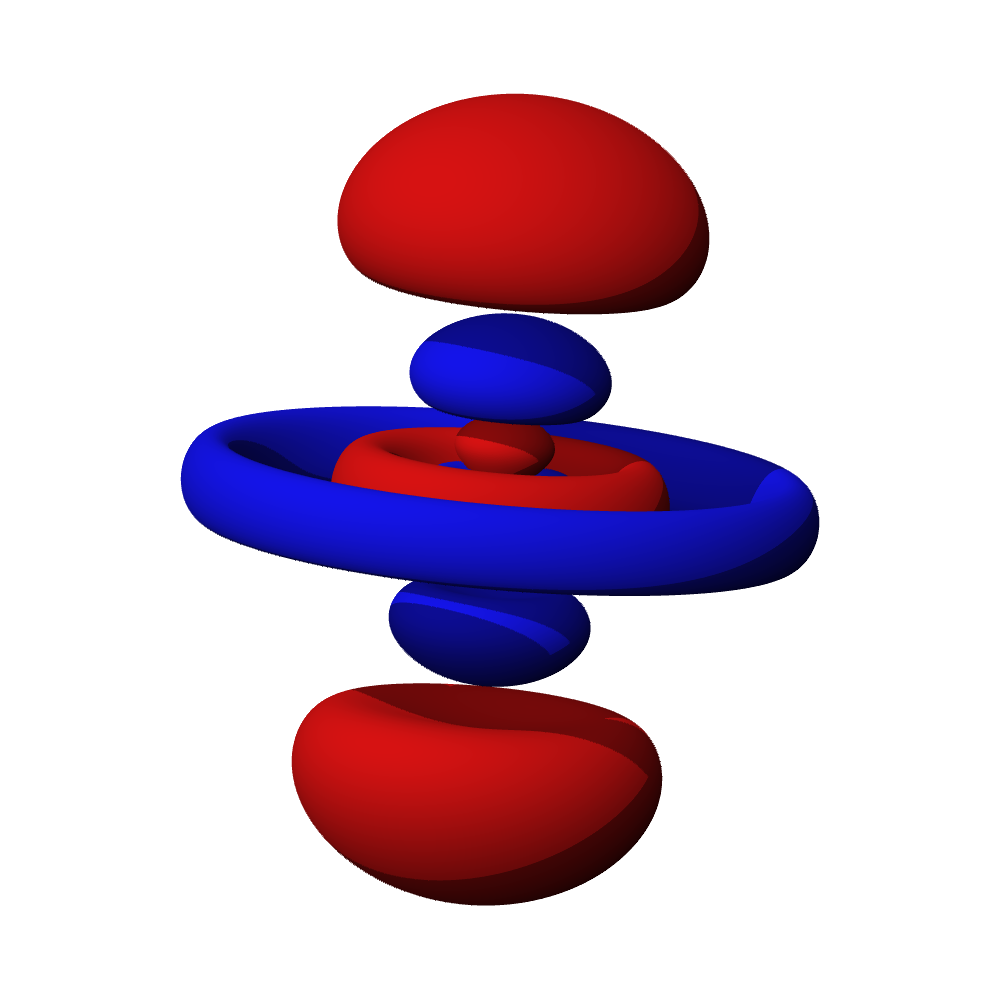
\includegraphics[width=1.6cm]{tableau_geometrie_orbitale_modelisation/D5z2.png} 
&
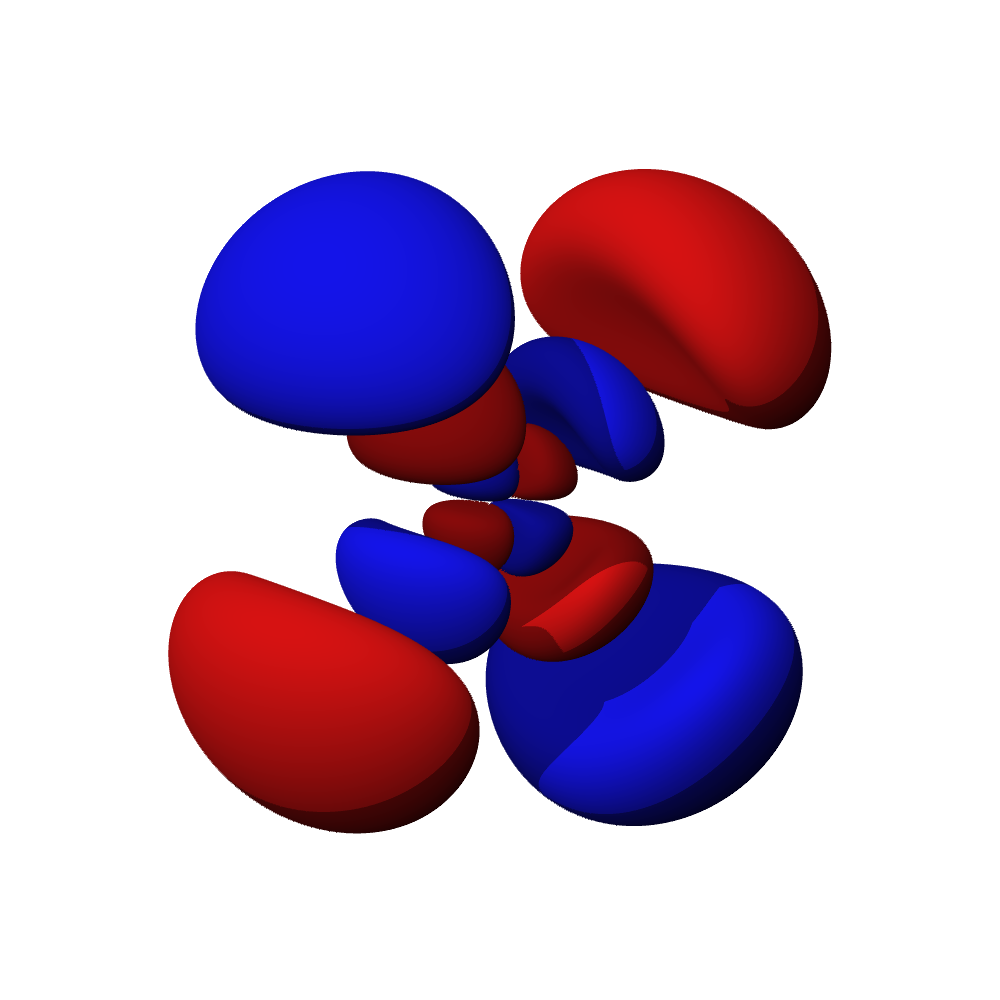
\includegraphics[width=1.6cm]{tableau_geometrie_orbitale_modelisation/D5xz.png}  
&
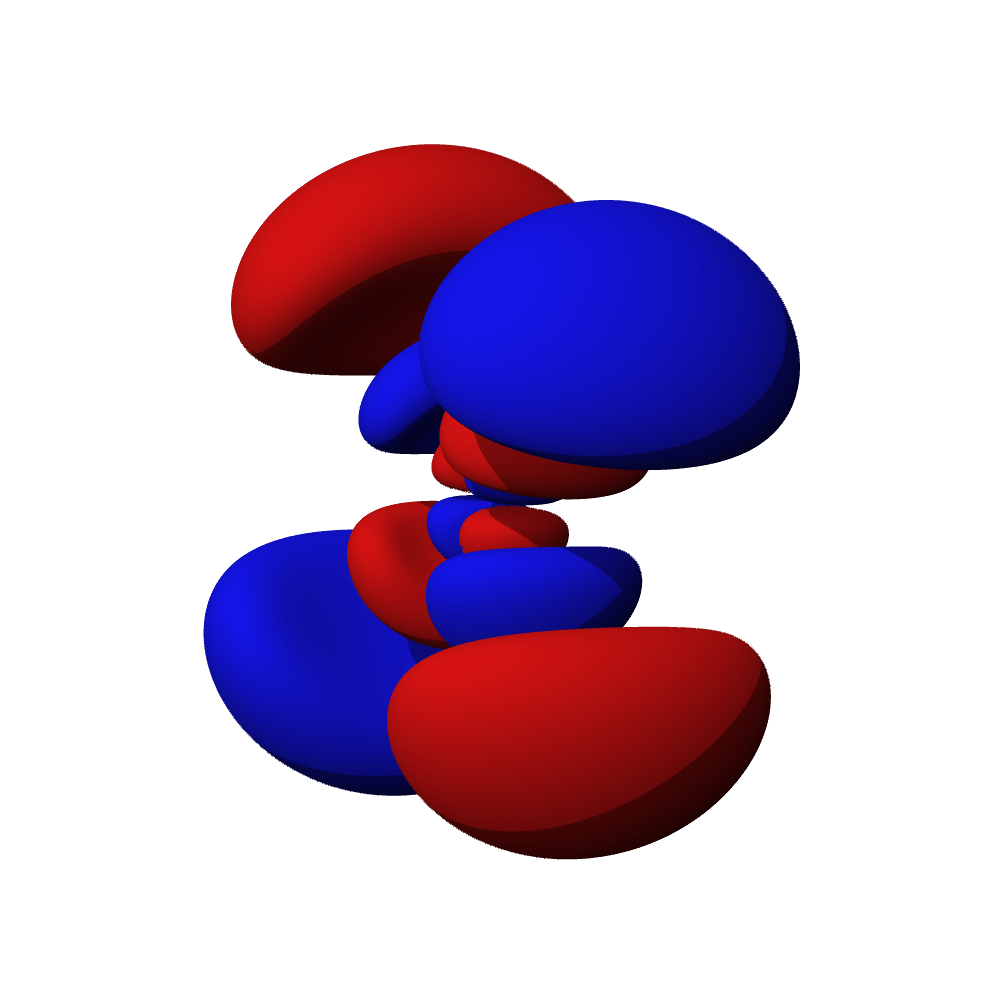
\includegraphics[width=1.6cm]{tableau_geometrie_orbitale_modelisation/D5yz.png} 
& 
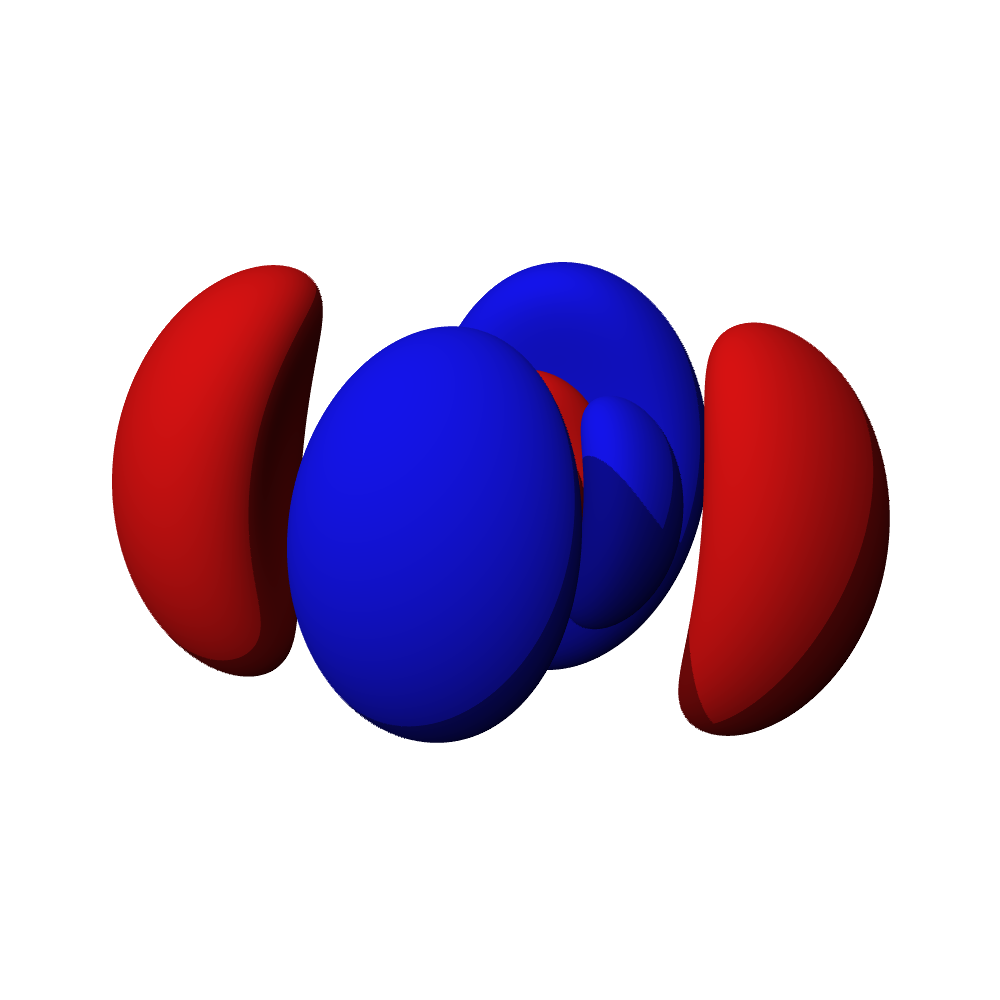
\includegraphics[width=1.6cm]{tableau_geometrie_orbitale_modelisation/D5xy.png} 
&
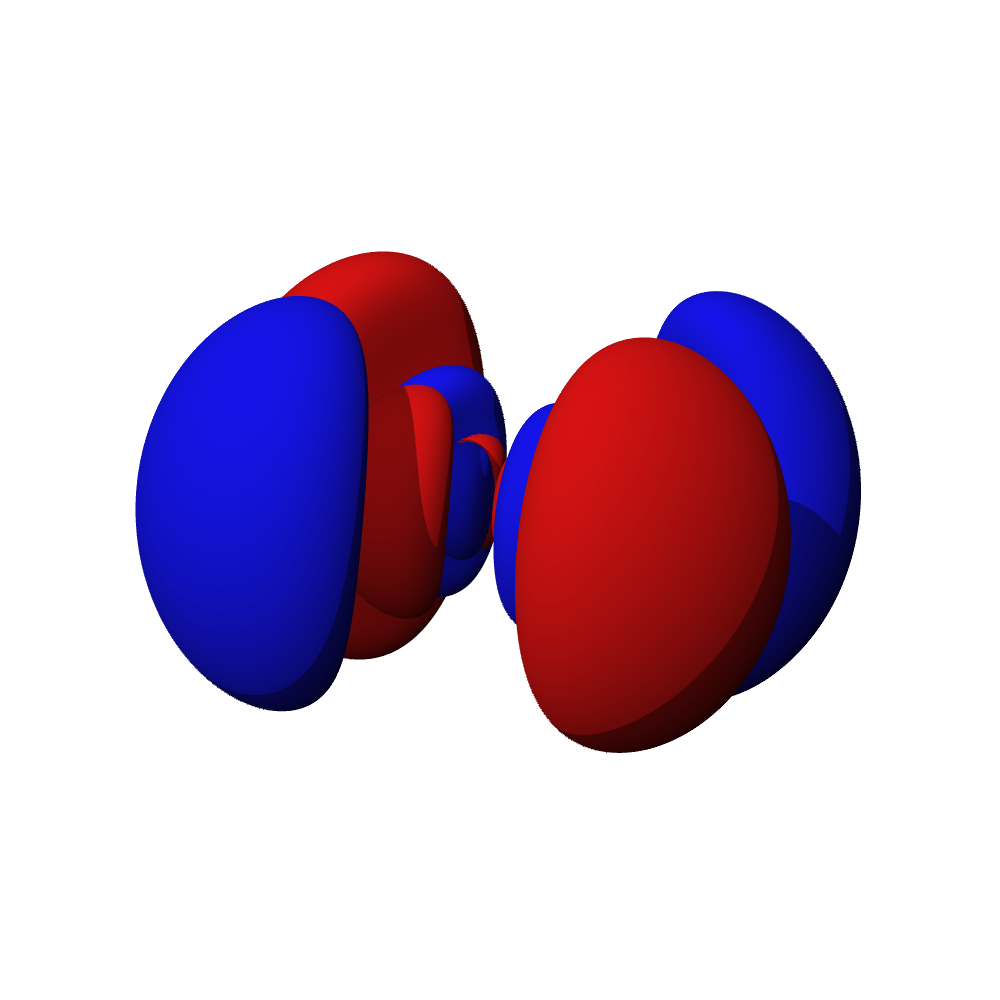
\includegraphics[width=1.6cm]{tableau_geometrie_orbitale_modelisation/D5x2-y2.png} 
& & \\
& & & \makecell[c]{$5d_{z^2}$} & \makecell[c]{$5d_{xz}$} & \makecell[c]{$5d_{yz}$} & \makecell[c]{$5d_{xy}$} & \makecell[c]{$5d_{x^{2}-y^{2}}$} & &  \\ %centrer la cellule individuellement 

\midrule

\multirow[t]{6}{*}{$n=6$} & \multirow[t]{2}{*}{$\ell=0$} & \multirow[t]{2}{*}{$6s$} & 
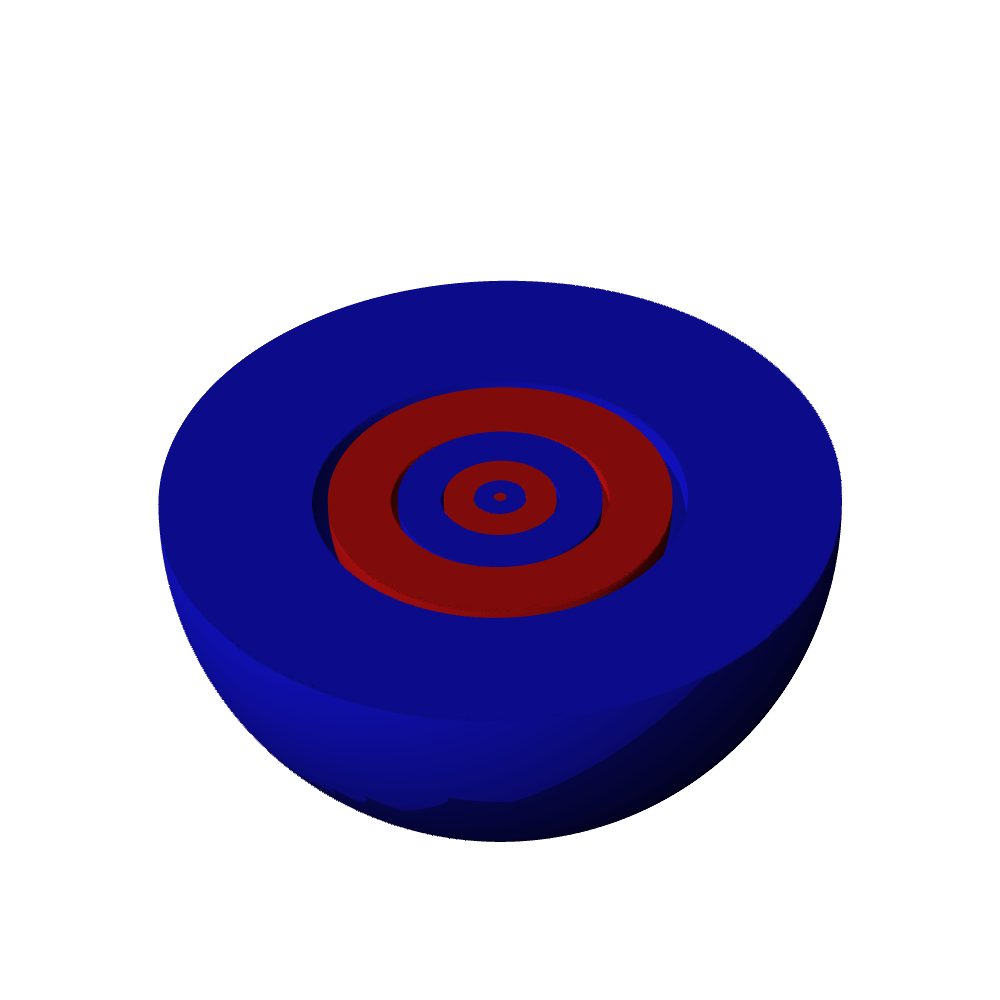
\includegraphics[width=1.6cm]{tableau_geometrie_orbitale_modelisation/S6M0.png} 
& & & & & & \\

& & & \makecell[c]{$6s$} & & & & & &  \\ %centrer la cellule individuellement 

\addlinespace

& \multirow[t]{2}{*}{$\ell=1$} & \multirow[t]{2}{*}{$6p$} & 
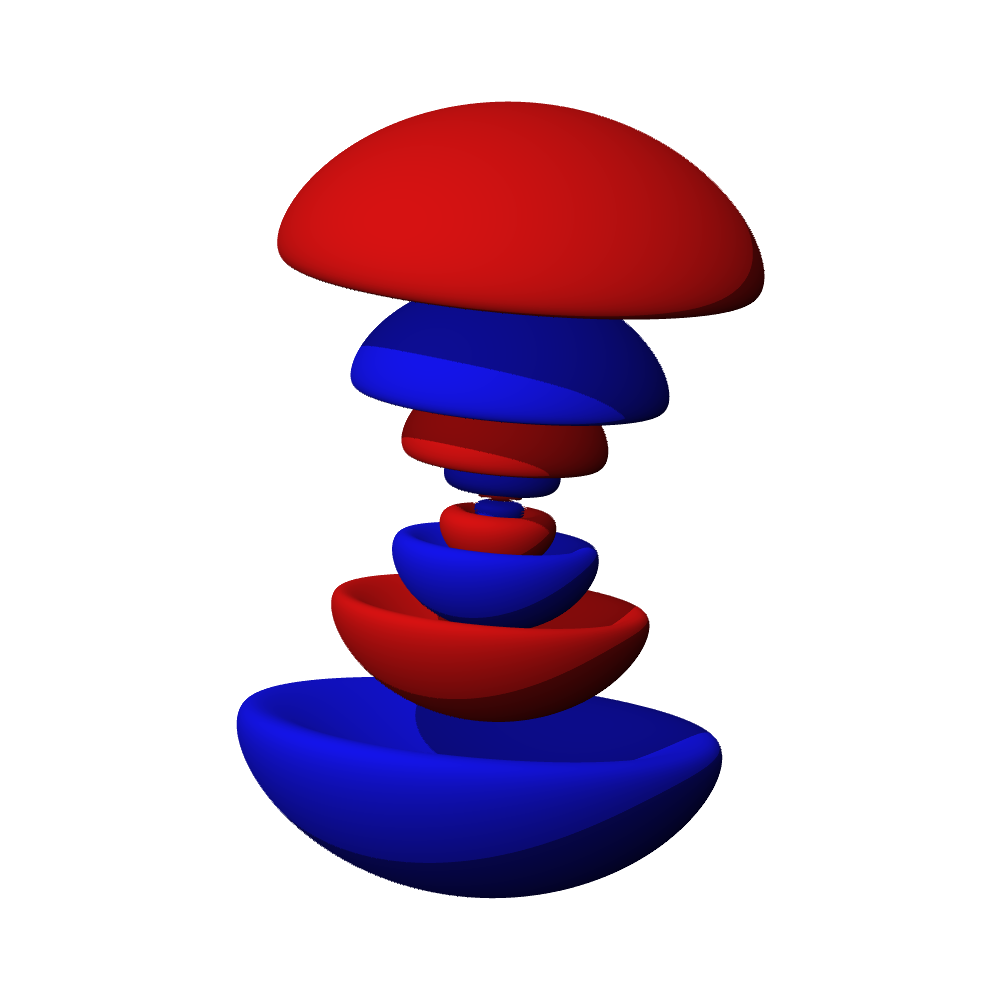
\includegraphics[width=1.6cm]{tableau_geometrie_orbitale_modelisation/P6z.png} 
&
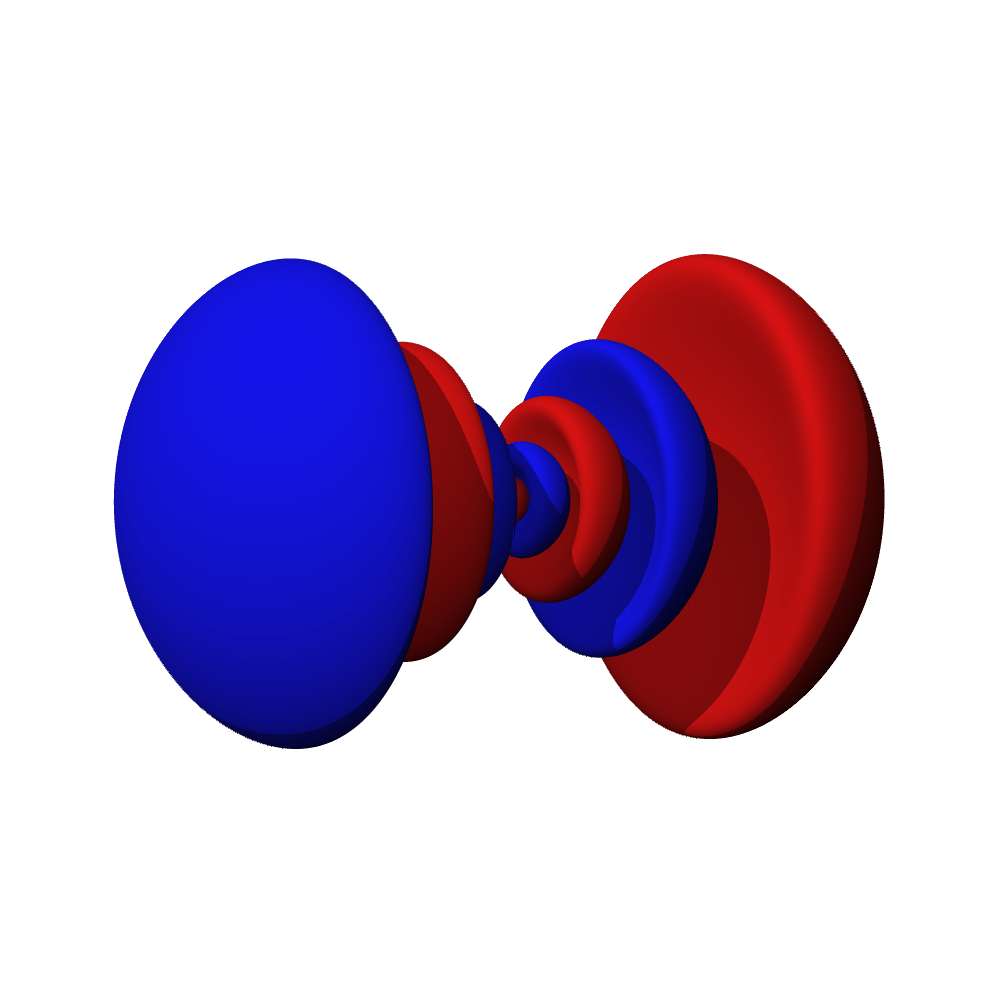
\includegraphics[width=1.6cm]{tableau_geometrie_orbitale_modelisation/P6x.png}  
&
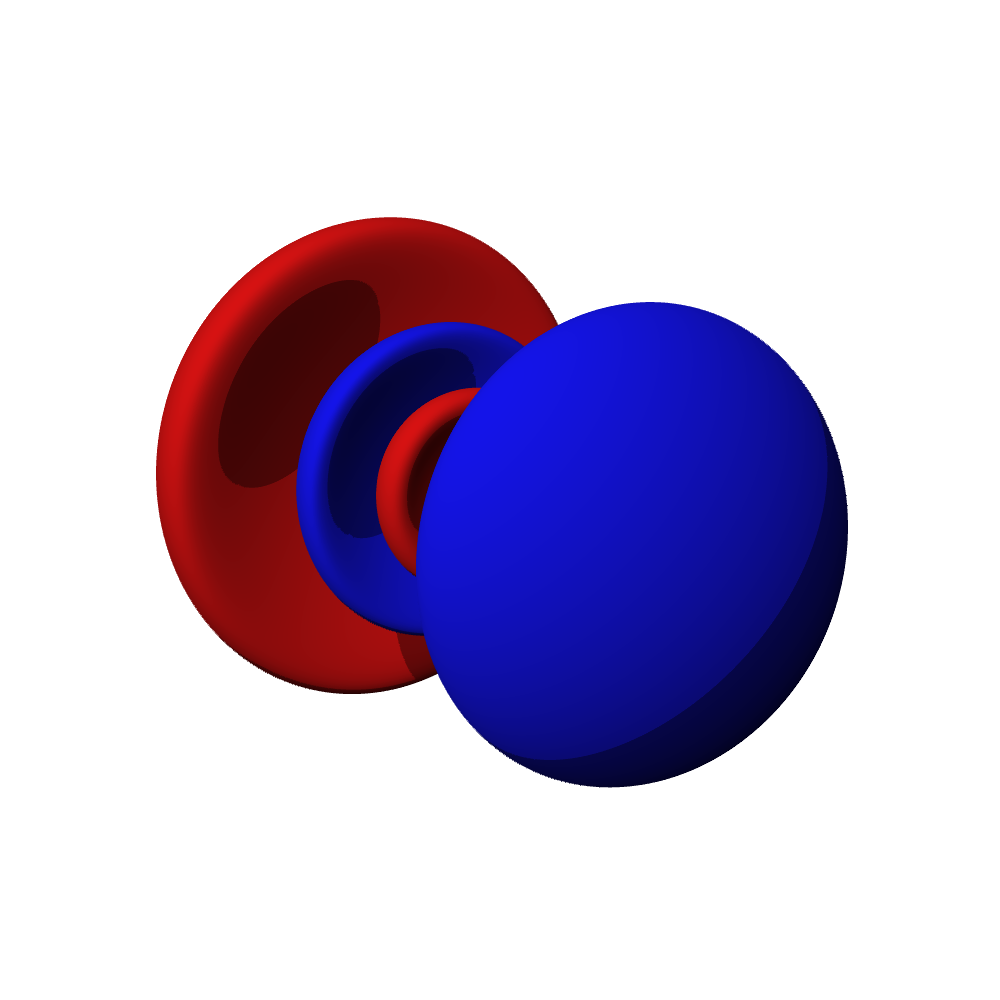
\includegraphics[width=1.6cm]{tableau_geometrie_orbitale_modelisation/P6y.png} 
& & & & \\

& & & \makecell[c]{$6p_z$} & \makecell[c]{$6p_x$} & \makecell[c]{$6p_y$} & & & &  \\ %centrer la cellule individuellement 

\addlinespace

 & \multirow[t]{2}{*}{$\ell=2$} & \multirow[t]{2}{*}{$6d$} & 
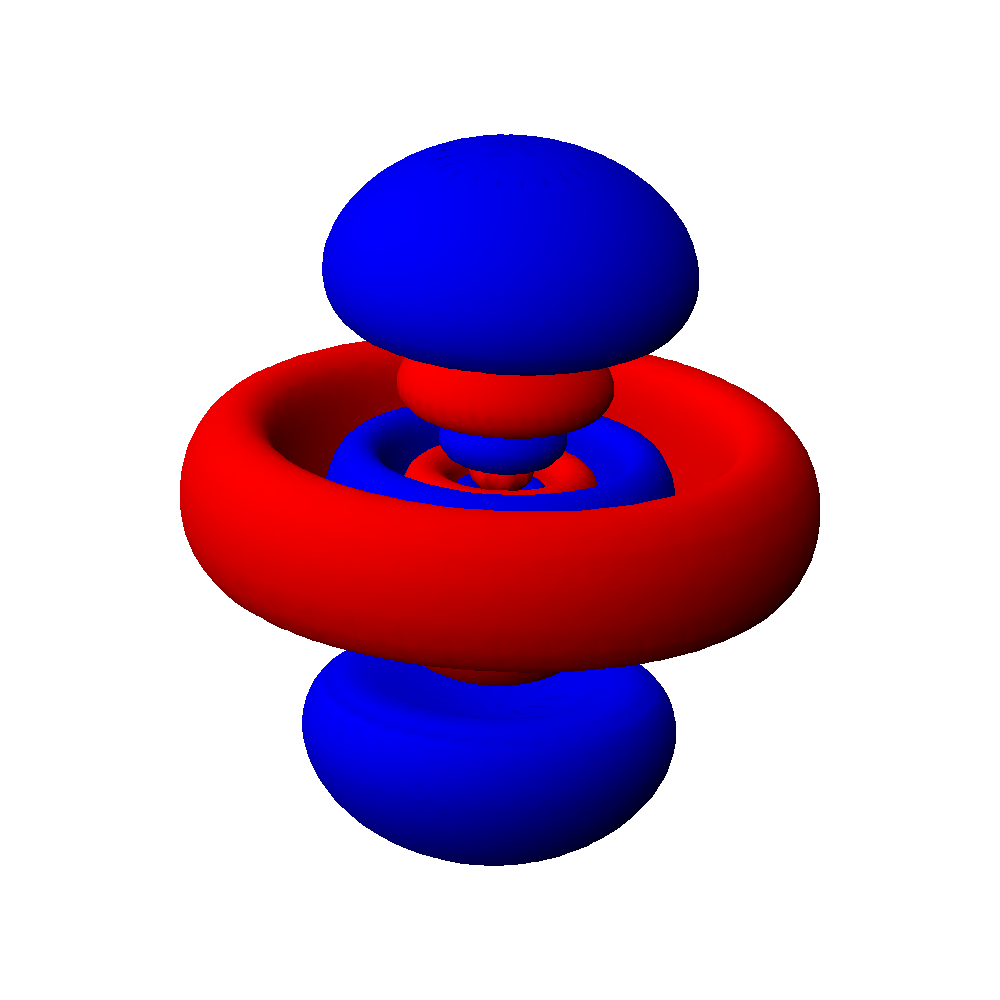
\includegraphics[width=1.6cm]{tableau_geometrie_orbitale_modelisation/D6z2.png} 
&
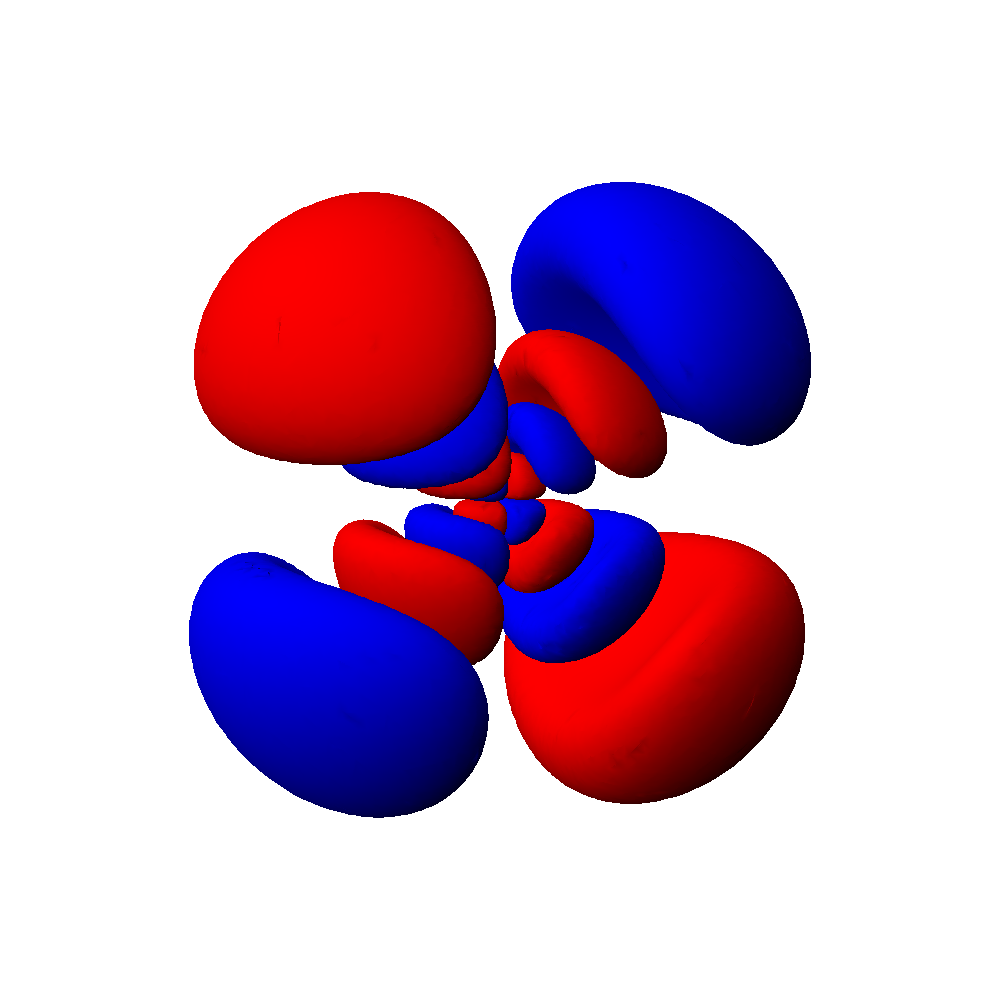
\includegraphics[width=1.6cm]{tableau_geometrie_orbitale_modelisation/D6xz.png}  
&
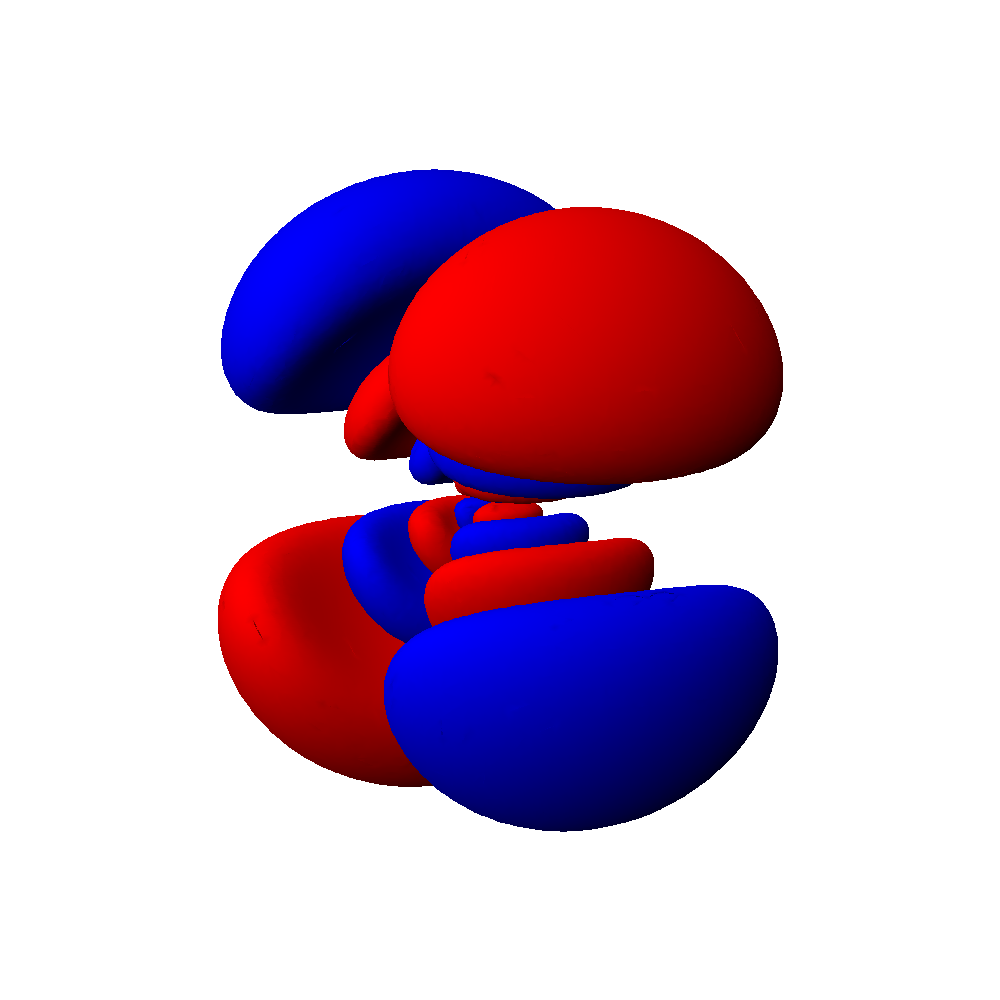
\includegraphics[width=1.6cm]{tableau_geometrie_orbitale_modelisation/D6yz.png} 
& 
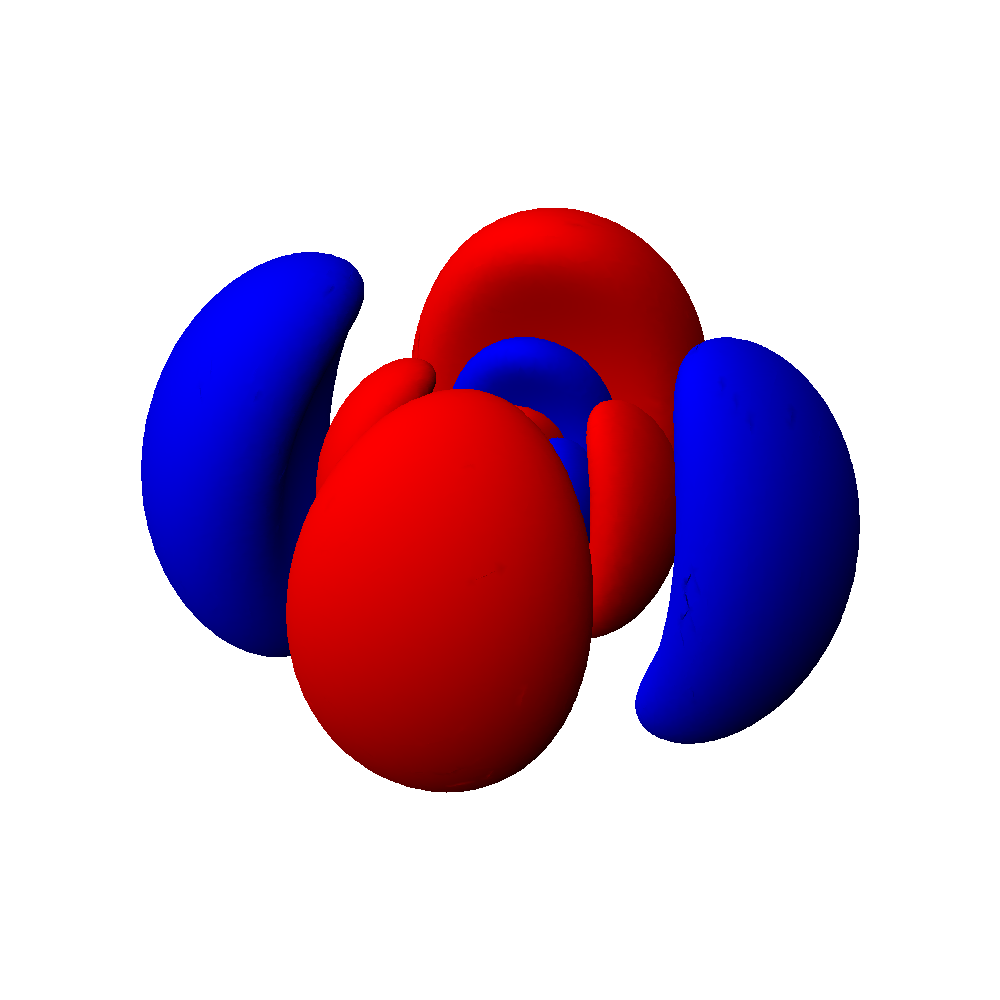
\includegraphics[width=1.6cm]{tableau_geometrie_orbitale_modelisation/D6xy.png} 
&
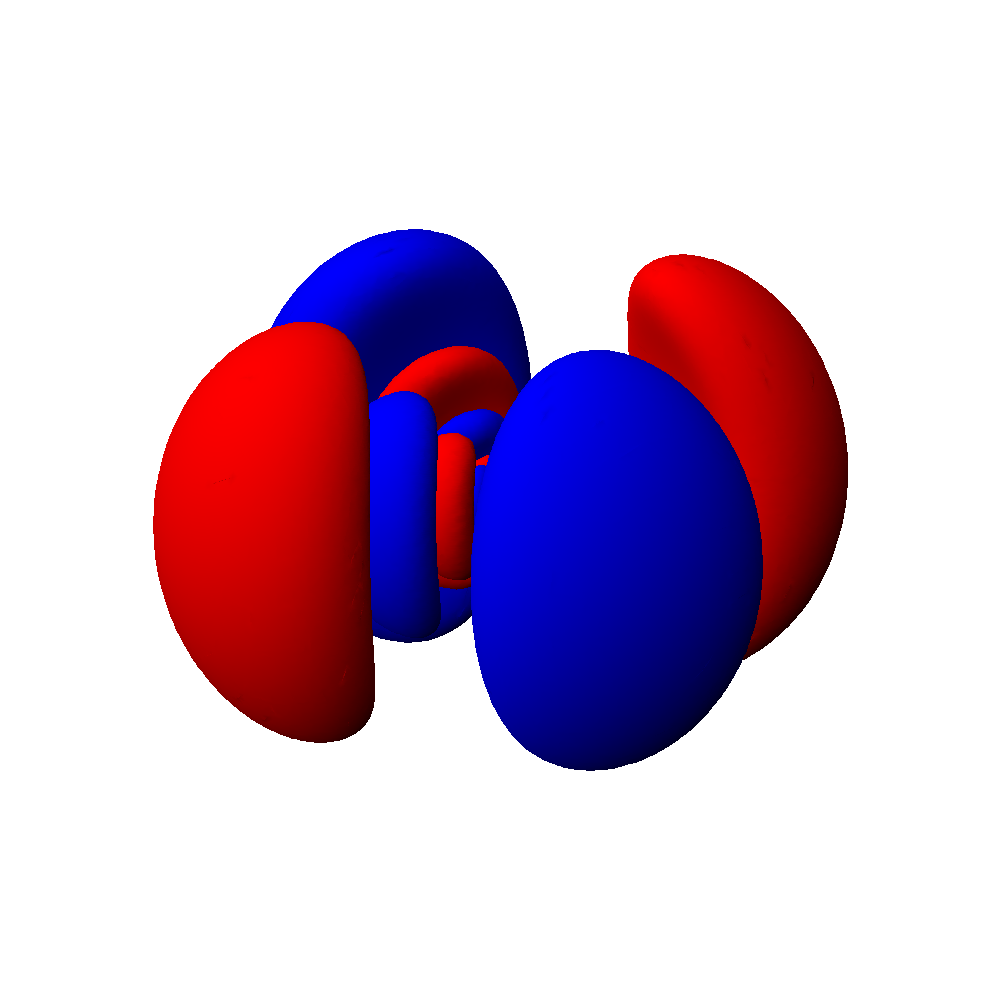
\includegraphics[width=1.6cm]{tableau_geometrie_orbitale_modelisation/D6x2-y2.png} 
& & \\
& & & \makecell[c]{$6d_{z^2}$} & \makecell[c]{$6d_{xz}$} & \makecell[c]{$6d_{yz}$} & \makecell[c]{$6d_{xy}$} & \makecell[c]{$6d_{x^{2}-y^{2}}$} & &  \\ %centrer la cellule individuellement 

\midrule

\multirow[t]{2}{*}{$n=7$} & \multirow[t]{2}{*}{$\ell=0$} & \multirow[t]{2}{*}{$7s$} & 
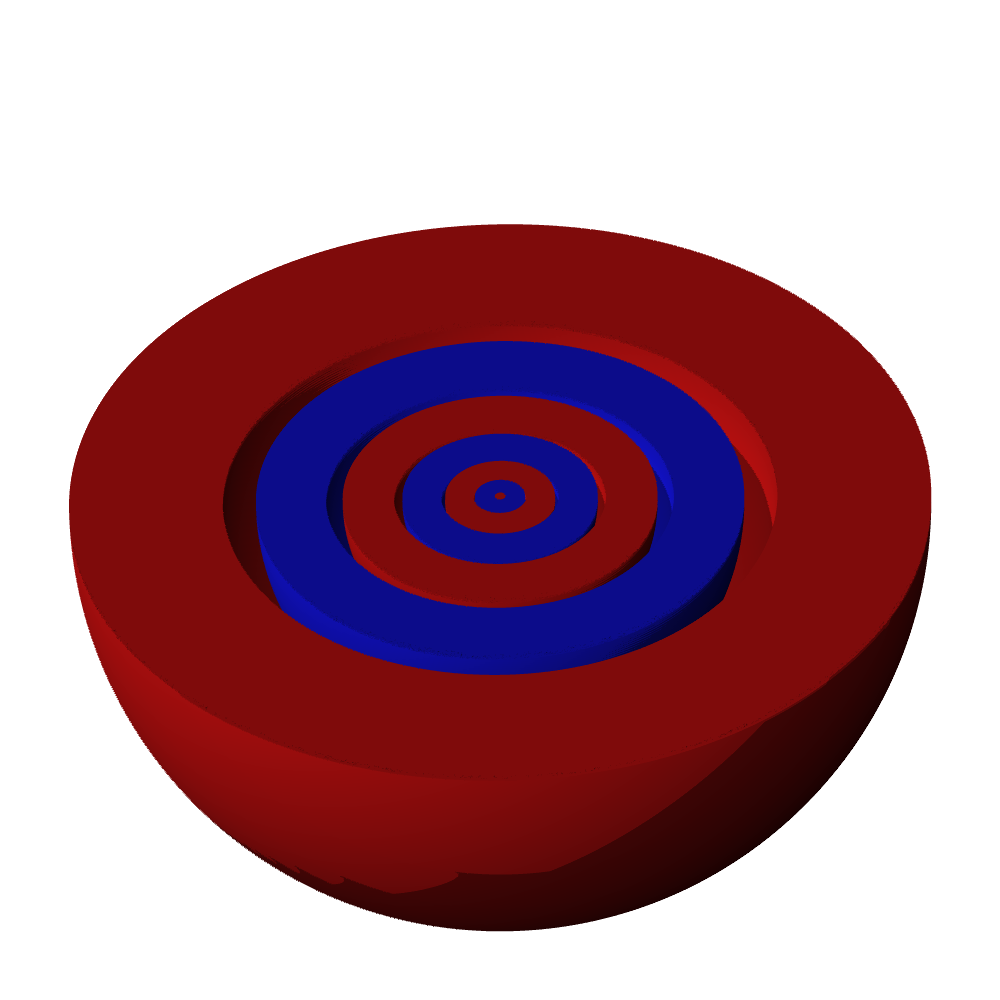
\includegraphics[width=1.6cm]{tableau_geometrie_orbitale_modelisation/S7M0.png} 
& & & & & & \\

& & & \makecell[c]{$7s$} & & & & & &  \\ %centrer la cellule individuellement 

\bottomrule

\end{xltabular}
\end{landscape}

%end{document}
